\documentclass[10pt,a4paper]{article}

\usepackage[T1]{fontenc}
\usepackage[utf8]{inputenc}
\usepackage{libertinus}
\usepackage[a4paper,margin=24mm,headheight=14pt]{geometry}
\usepackage{microtype}
\usepackage{graphicx}
\usepackage{mathtools,amssymb,amsthm,bm}
\usepackage{booktabs,longtable,array,tabularx,multirow}
\usepackage{enumitem}
\usepackage[dvipsnames]{xcolor}
\usepackage{tikz}
\usetikzlibrary{arrows.meta,positioning,calc,fit,shapes.geometric,backgrounds}
\usepackage[most]{tcolorbox}
\usepackage{listings}
\usepackage{fvextra}
\usepackage{fancyhdr}
\usepackage{caption}
\usepackage{subcaption}
\usepackage[hidelinks]{hyperref}
\usepackage[nameinlink,noabbrev]{cleveref}
\usepackage{xurl}
\usepackage{setspace}

\setstretch{1.045}
\raggedbottom
\setlength{\emergencystretch}{3em}
\setlength{\parindent}{1.25em}
\setlength{\parskip}{0.16em}
\setlist[itemize]{leftmargin=1.55em,itemsep=0.18em,topsep=0.28em}
\setlist[enumerate]{leftmargin=1.85em,itemsep=0.18em,topsep=0.28em}
\renewcommand{\arraystretch}{1.12}

\definecolor{DeepBlue}{HTML}{163B65}
\definecolor{MidBlue}{HTML}{2D5F8B}
\definecolor{LightBlue}{HTML}{EAF2F8}
\definecolor{DeepRed}{HTML}{8D2534}
\definecolor{LightRed}{HTML}{F9ECEF}
\definecolor{DeepGreen}{HTML}{2E604A}
\definecolor{LightGreen}{HTML}{EDF6F1}
\definecolor{DarkGray}{HTML}{333333}
\definecolor{RuleGray}{HTML}{CDD4DB}
\definecolor{TickleOrange}{HTML}{F39C34}

\hypersetup{
  pdftitle={The Mr Tickle Screen: a reductio against physical closure from bare observer screens},
  pdfauthor={Open Technical Audit contributors},
  pdfsubject={A reductio ad absurdum against physical closure from bare observer screens},
  colorlinks=true,
  linkcolor=DeepBlue,
  citecolor=DeepBlue,
  urlcolor=MidBlue
}

\pagestyle{fancy}
\fancyhf{}
\fancyhead[L]{\small\textsc{The Mr Tickle Screen}}
\fancyhead[R]{\small Anonymous technical audit \textbullet\ 26 August 2026}
\fancyfoot[C]{\small\thepage}
\renewcommand{\headrulewidth}{0.35pt}

\newtheorem{theorem}{Theorem}[section]
\newtheorem{lemma}[theorem]{Lemma}
\newtheorem{proposition}[theorem]{Proposition}
\newtheorem{corollary}[theorem]{Corollary}
\newtheorem{noescape}[theorem]{No-escape theorem}
\newtheorem{reductio}[theorem]{Reductio}
\theoremstyle{definition}
\newtheorem{definition}[theorem]{Definition}
\newtheorem{assumption}[theorem]{Assumption}
\newtheorem{example}[theorem]{Example}
\theoremstyle{remark}
\newtheorem{remark}[theorem]{Remark}

\newtcolorbox{summarybox}[1][]{
  enhanced,breakable,colback=LightBlue,colframe=DeepBlue,
  boxrule=0.7pt,arc=1mm,left=2.4mm,right=2.4mm,top=1.8mm,bottom=1.8mm,
  title=#1,fonttitle=\bfseries
}
\newtcolorbox{resultbox}[1][]{
  enhanced,breakable,colback=LightGreen,colframe=DeepGreen,
  boxrule=0.7pt,arc=1mm,left=2.4mm,right=2.4mm,top=1.8mm,bottom=1.8mm,
  title=#1,fonttitle=\bfseries
}
\newtcolorbox{warningbox}[1][]{
  enhanced,breakable,colback=LightRed,colframe=DeepRed,
  boxrule=0.7pt,arc=1mm,left=2.4mm,right=2.4mm,top=1.8mm,bottom=1.8mm,
  title=#1,fonttitle=\bfseries
}
\newtcolorbox{proofbox}[1][]{
  enhanced,breakable,colback=white,colframe=RuleGray,
  boxrule=0.55pt,arc=1mm,left=2.4mm,right=2.4mm,top=1.8mm,bottom=1.8mm,
  title=#1,fonttitle=\bfseries\color{DarkGray}
}

\lstdefinelanguage{Lean}{
  morekeywords={def,theorem,lemma,structure,class,namespace,end,where,by,intro,exact,
    apply,have,show,from,let,in,if,then,else,match,with,fun,forall,exists,
    variable,universe,open,import,rcases,constructor,calc,simpa,using},
  sensitive=true,
  morecomment=[l]{--},
  morecomment=[s]{/-}{-/},
  morestring=[b]"
}
\lstset{
  language=Lean,
  basicstyle=\ttfamily\footnotesize,
  keywordstyle=\color{DeepBlue}\bfseries,
  commentstyle=\color{DeepGreen},
  stringstyle=\color{DeepRed},
  columns=fullflexible,
  keepspaces=true,
  breaklines=true,
  frame=single,
  rulecolor=\color{RuleGray},
  backgroundcolor=\color{black!1},
  xleftmargin=1mm,
  xrightmargin=1mm,
  showstringspaces=false
}

\newcommand{\OPH}{\mathrm{OPH}}
\newcommand{\Lsrc}{L_{\mathrm{src}}}
\newcommand{\Lphys}{L_{\mathrm{phys}}}
\newcommand{\Tsrc}{T_{\mathrm{src}}}
\newcommand{\Mod}{\operatorname{Mod}}
\newcommand{\Red}{\operatorname{Red}}
\newcommand{\Obs}{\mathcal O}
\newcommand{\Phys}{\mathsf{Phys}}
\newcommand{\Src}{\mathsf{Src}}
\newcommand{\Real}{\operatorname{Real}}
\newcommand{\im}{\operatorname{im}}
\newcommand{\id}{\mathrm{id}}
\newcommand{\defeq}{\mathrel{:=}}
\newcommand{\obsim}{\sim_{\Obs}}
\newcommand{\gaugesim}{\sim_{\mathrm g}}
\newcommand{\restr}{\mathord{\upharpoonright}}
\newcommand{\notmodels}{\mathrel{\not\models}}

\begin{document}
\pagenumbering{roman}

\begin{titlepage}
\thispagestyle{empty}
\noindent{\color{DeepBlue}\rule{\textwidth}{1.2pt}}\\[7mm]
{\small\bfseries\color{DeepBlue} RESEARCH ARTICLE \hfill 26 AUGUST 2026}\\[12mm]
{\Huge\bfseries The Mr Tickle Screen\par}
\vspace{4mm}
{\Large A reductio ad absurdum against physical closure from bare observer screens\par}
\vspace{5mm}
{\large No Semantic Alchemy, No Bulk From Bare Boundary, and physical non-definability in Observer Patch Holography\par}
\vspace{12mm}
{\large Anonymous technical audit\par}
{\normalsize Authorship intentionally withheld in the public package\par}
\vspace{12mm}

\begin{summarybox}[Central result]
Assume that a source-only observer-screen architecture is sufficient to make
its formal screen a physically instantiated holographic boundary and to select
a physical bulk.  Then any source-isomorphic presentation---including the
``Mr Tickle Screen'' constructed below---inherits the same alleged physical
status.  But source mathematics cannot constrain an external physical-
realization relation: the same source model admits an expansion in which that
relation is empty.  Moreover, a bare twelve-port incidence structure does not
determine the boundary quantum theory required by a holographic dictionary.
Therefore physical closure cannot be obtained from A1--A3, nor from any
purely source-internal enrichment of them.  A successful future closure must
supply independently grounded physical boundary dynamics and a reconstruction
dictionary; once supplied, those are additional load-bearing physical
structure rather than consequences of the bare screen alone.
\end{summarybox}

\vfill
\noindent\textbf{Frozen audit baseline.} FloatingPragma/observer-patch-holography,
commit\\
\texttt{40b13bb4bc56261f84fd515701916c388c42fe83}.\\[2mm]
\noindent\textbf{Live public snapshot checked.} Main-branch commit\\
\texttt{05207466cf63461c683bf1b8543d7c4a5feea4fa} (26 August 2026).\\[2mm]
\noindent\textbf{Priority statement.} The source/realization countermodel was
documented in a hash-anchored prior audit dated 2 August 2026.  The present article generalizes that witness
into a source-only physical-closure impossibility theorem, a holographic typing
obstruction, and a Lean 4 proof kernel.\\[2mm]
\noindent\textbf{Scope.} Internal source theorems may remain correct.  The claim
under attack is that source formalism, observer consensus, or theorem volume
can by themselves establish physical instantiation or a unique physical bulk.

\vspace{8mm}
\noindent{\color{DeepBlue}\rule{\textwidth}{1.2pt}}
\end{titlepage}
\pagenumbering{arabic}

\begin{abstract}
We present a reductio ad absurdum against deriving physical ontology from a
bare observer-screen formalism.  The reductio is intentionally simple.  Let a
source theory characterize an abstract screen, records, overlaps, agreement,
response algebras, fixed points and an information-projection rule.  Assume,
for contradiction, that satisfaction of those source conditions is sufficient
to establish that the screen is physically instantiated and that a physical
bulk is thereby selected.  Because the source theory is presentation-
invariant, an isomorphic source model can be displayed on an arbitrary
pictorial carrier.  We choose an original long-armed orange cartoon schematic,
the ``Mr Tickle Screen'', carrying the same formal twelve-port source data.  If
source structure alone established physicality, the cartoon presentation
would inherit that status.  The absurd conclusion reveals the missing type:
physical instantiation is not a source-language property.  Formally, a
satisfiable source theory admits an expansion with an empty external
realization relation; therefore no source-only enrichment can force external
physical realization.  We call this result \emph{No Semantic Alchemy}.

A second, independent obstruction comes from holography.  AdS/CFT and HKLL do
not reconstruct a bulk from bare boundary incidence.  They act on a specified
boundary quantum theory with operator algebra, states, dynamics and
correlators, together with a duality/reconstruction dictionary.  The same
finite twelve-site carrier can support inequivalent Hamiltonians and
correlation structures, so the bare screen cannot uniquely select the
boundary theory that a holographic reconstruction requires.  We formalize the
result as \emph{No Bulk From Bare Boundary}: if two boundary theories share the
same bare screen but have different reconstruction outputs, no bulk assignment
can factor through the bare screen alone.  Combining these results with the
previous same-reduct physical non-definability theorem yields a strict closure
dichotomy for Observer Patch Holography (OPH): remain source-only and physical
closure is impossible; or introduce independently grounded physical boundary
dynamics, calibration and a holographic dictionary, in which case those
objects are additional load-bearing physical structure and the closure is no
longer a consequence of A1--A3 alone.  The theorem is independent of the
number of machine-checked source consequences.
\end{abstract}

\begin{summarybox}[One-sentence reductio]
If the same formal criteria that supposedly make an OPH screen physically
fundamental can be carried unchanged by the Mr Tickle Screen, then either the
cartoon has become a physical holographic boundary or those criteria were
never sufficient to establish physicality.  Formal annotation does not
instantiate its referent, so the second horn follows.
\end{summarybox}

\tableofcontents
\clearpage

\section{Introduction: why the absurdity is the argument}

The central error audited here is a type error between \emph{characterizing a
formal object} and \emph{establishing that nature instantiates it}.  The error
can hide for a long time when the formal vocabulary uses physical nouns.
Calling mathematical objects ``observers'', ``screens'', ``records'',
``currents'', ``repair'', ``meaning'', ``horizons'' or ``bulk'' does not turn
those objects into laboratory systems.  Nor does adding more internally valid
theorems.  Formal consistency is a relation among statements or structures;
physical occurrence is a relation between a mathematical representation and
the world.

The point becomes obvious under a deliberately absurd presentation.  Take a
source model satisfying every relevant formal condition and draw its carrier
on a long-armed orange cartoon figure.  Call this the \emph{Mr Tickle Screen}.
The artwork is irrelevant: the abstract source model is unchanged.  If one
claims that the source conditions themselves are sufficient to make the
screen physically instantiated, then the same implication applies to this
presentation.  The conclusion is absurd not because cartoons cannot support
mathematics, but because mathematics attached to a cartoon does not cause the
cartoon to occur in nature.  The only information used to reject the physical
Mr Tickle Screen is information external to the source formalism---precisely
the missing physical-realization content.

This reductio is then made exact in three steps.  First, standard reduct/
expansion machinery shows that a satisfiable source theory cannot force an
external realization relation: the empty relation is always a same-source
expansion unless physical realization has been imported into the premises.
Second, factorization theory shows that a bare screen cannot determine a
boundary quantum theory when two inequivalent boundary dynamics live on the
same screen.  Third, the holographic dictionary is typed from a specified
boundary theory to a bulk description; a screen is not the required input.
Thus no source-only theorem can jump directly from incidence/consensus to a
physical bulk.

The target is not a caricature of holography.  In AdS/CFT, the boundary side
is a specified conformal quantum field theory and the bulk side is a specified
gravity/string theory.  Maldacena's proposal and Witten's generating-
functional dictionary relate those two theories~\cite{Maldacena1997,Witten1998}.
HKLL then represents local bulk fields by nonlocal boundary operators in the
semiclassical regime~\cite{HKLL2006}; modern bulk reconstruction can also be
formulated in quantum-error-correcting language~\cite{ADH2015}.  None of this
says that drawing a boundary creates a bulk.  It says that, given a physical
boundary theory and a valid duality dictionary, bulk observables can be
reconstructed from boundary data.

\subsection{What is borrowed and what is new}

The machinery is standard: reducts and expansions, model-theoretic
satisfaction, Beth definability, forgetful functors and factorization,
observational equivalence, gauge-invariant readouts, information projection,
and the established AdS/CFT/HKLL reconstruction architecture
\cite{Beth1953,Hodges1993,ChangKeisler,KullbackLeibler,Csiszar1975,Jaynes1957,Maldacena1997,Witten1998,HKLL2006,ADH2015}.

The new contribution is the composition of these tools into an explicit
reductio and a closure theorem.  The argument does not merely say that a
physical bridge is ``open''.  It proves that \emph{no bridge whose content
remains entirely inside the source language can perform the missing physical
work}.  If a later bridge supplies independent boundary dynamics, laboratory
calibration or a holographic dictionary, then it may be scientifically
valuable, but it is additional physical structure and must be counted as such.

\section{The Mr Tickle Screen reductio}
\label{sec:tickle}

\subsection{Construction}

Let \(T_S\) denote a source theory and let \(M\models T_S\).  In the OPH
application, \(M\) contains the twelve-port boundary packet, overlap/seam
structure, record and readback interfaces, response algebra, agreement maps,
and A3 state-selection data.  Let \(P\) denote a source presentation.  A
presentation change is admissible when it preserves every source object and
map that the theory treats as protected.

The Mr Tickle Screen is not a competing physical theory.  It is the same
abstract source model displayed on a deliberately ridiculous pictorial
carrier.  The point is to remove any accidental persuasive force contributed
by words such as ``screen'' or by a diagram that visually resembles a
scientific boundary.

\begin{figure}[htbp]
\centering
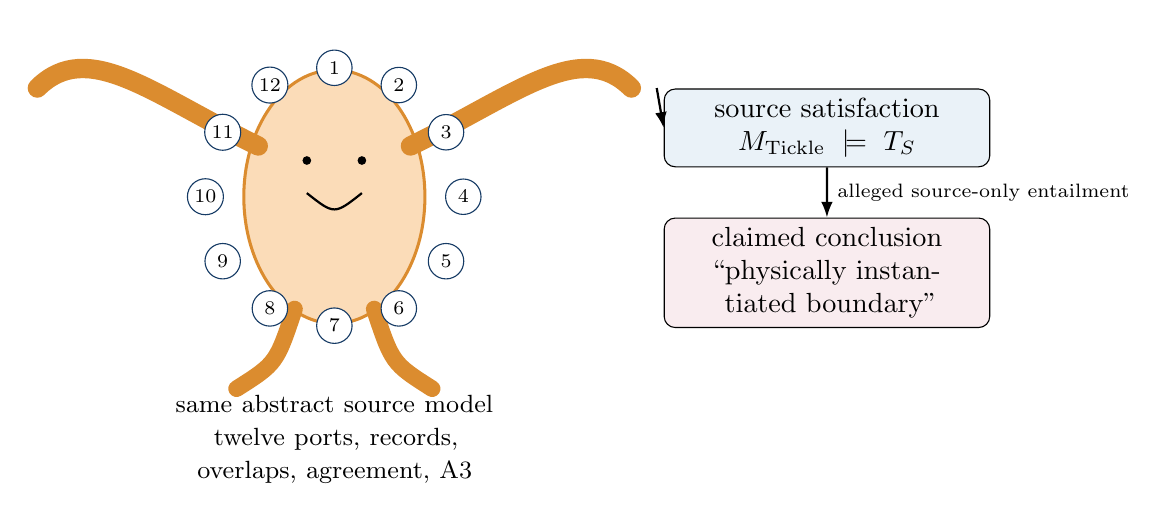
\begin{tikzpicture}[scale=0.92,
  port/.style={circle,draw=DeepBlue,fill=white,inner sep=1.4pt,minimum size=4.5mm},
  arr/.style={-{Latex[length=2mm]},thick}]
  % Original long-armed orange schematic; no publisher artwork is reproduced.
  \filldraw[fill=TickleOrange!35,draw=TickleOrange!90!black,line width=1.1pt]
    (0,0) ellipse (1.25 and 1.75);
  \draw[TickleOrange!90!black,line width=7pt,line cap=round]
    (-1.05,0.7) .. controls (-2.5,1.4) and (-3.4,2.2) .. (-4.1,1.5);
  \draw[TickleOrange!90!black,line width=7pt,line cap=round]
    (1.05,0.7) .. controls (2.5,1.4) and (3.4,2.2) .. (4.1,1.5);
  \draw[TickleOrange!90!black,line width=6pt,line cap=round]
    (-0.55,-1.55) .. controls (-0.8,-2.3) .. (-1.35,-2.65);
  \draw[TickleOrange!90!black,line width=6pt,line cap=round]
    (0.55,-1.55) .. controls (0.8,-2.3) .. (1.35,-2.65);
  \fill ( -0.38,0.50) circle (0.06); \fill (0.38,0.50) circle (0.06);
  \draw[line width=0.8pt] (-0.38,0.05) .. controls (0,-0.25) .. (0.38,0.05);
  % Twelve abstract ports: same formal payload, silly presentation.
  \foreach \a/\lab in {90/1,60/2,30/3,0/4,-30/5,-60/6,-90/7,-120/8,-150/9,180/10,150/11,120/12}{
    \node[port] (p\lab) at ({1.78*cos(\a)},{1.78*sin(\a)}) {\scriptsize\lab};
  }
  \node[align=center,text width=48mm] at (0,-3.35)
    {\small same abstract source model\\twelve ports, records, overlaps, agreement, A3};
  \node[draw,rounded corners,fill=LightBlue,align=center,text width=39mm] (formal) at (6.8,0.95)
    {source satisfaction\\\(M_{\rm Tickle}\models T_S\)};
  \node[draw,rounded corners,fill=LightRed,align=center,text width=39mm] (physical) at (6.8,-1.05)
    {claimed conclusion\\``physically instantiated boundary''};
  \draw[arr] (4.45,1.5) -- (formal.west);
  \draw[arr] (formal) -- node[right,font=\scriptsize]{alleged source-only entailment} (physical);
\end{tikzpicture}
\caption{The Mr Tickle Screen reductio.  The cartoon is an original schematic
used for criticism/parody; it does not reproduce published Mr. Men artwork.
The source-theoretic point is independent of appearance: a presentation can
carry the same abstract mathematics without acquiring physical instantiation.
Only the port locations are sketched; the full abstract 30-edge/20-face packet
is unchanged and is not redrawn on the cartoon.}
\label{fig:tickle}
\end{figure}

\subsection{Reductio ad absurdum}

Assume for contradiction that source satisfaction is sufficient for physical
instantiation:
\begin{equation}
\label{eq:bad-entailment}
M\models T_S
\quad\Longrightarrow\quad
\operatorname{PhysReal}(M).
\end{equation}
If \(M_{\rm Tickle}\) is source-isomorphic to \(M\), then every
presentation-invariant source theorem has the same truth value on both.  The
assumption \eqref{eq:bad-entailment} therefore yields
\[
\operatorname{PhysReal}(M_{\rm Tickle}).
\]
But no pictorial recoding, no matter how mathematically elaborate, creates a
new physical object.  The rejection of that conclusion must appeal to facts
outside the source presentation.  Therefore the source structure was not
sufficient for physical instantiation in the first place.

\begin{reductio}[Mr Tickle Screen]
Let \(T_S\) be presentation-invariant and satisfiable.  If physical
instantiation is not itself fixed by the source language, then source
satisfaction cannot entail physical instantiation.  In particular, replacing
a scientific-looking presentation by the Mr Tickle Screen cannot change any
source theorem but also cannot create a physical boundary.  Hence any rule
that promotes the former but not the latter must consume additional
non-source information.
\end{reductio}

\begin{warningbox}[Why the joke is mathematically useful]
The reductio does not argue that a fictional character is a model of physics.
It argues that \emph{formal annotation is not an ontological creation
operator}.  A cartoon can carry a graph, an algebra, a probability law and an
arbitrarily large theorem library.  Those properties remain properties of the
formal representation until an independently grounded physical-realization
relation is established.
\end{warningbox}

\section{No Semantic Alchemy}
\label{sec:alchemy}

Let \(L_S\) be the source language and let \(T_S\) be a satisfiable theory in
that language.  Introduce a distinct relation
\[
\mathcal R\subseteq \Mod(T_S)\times\mathcal W,
\]
where \(\mathcal R(M,w)\) means that source model \(M\) is physically
instantiated by world/system \(w\).  The relation is intentionally external to
\(L_S\): it expresses the representation-to-world fact whose existence is at
issue.

\begin{theorem}[No Semantic Alchemy]
\label{thm:alchemy}
If \(T_S\) is satisfiable and contains no condition that fixes the external
relation \(\mathcal R\), then
\[
T_S\notmodels \exists w\,\mathcal R(M,w).
\]
More strongly, for any source-only enrichment \(T_S^+=T_S\cup\Delta\) that
remains satisfiable and still does not constrain \(\mathcal R\),
\[
T_S^+\notmodels \exists w\,\mathcal R(M,w).
\]
\end{theorem}

\begin{proof}
Choose a source model \(M\models T_S^+\).  Form two expansions with the same
source reduct.  In the first, set \(\mathcal R=\varnothing\); in the second,
choose any nonempty realization relation.  Every \(L_S\)-sentence has the
same truth value in the two expansions because their source reducts are
identical.  The first expansion falsifies \(\exists w\,\mathcal R(M,w)\).
Therefore no source-only sentence can entail that existential claim.
\end{proof}

The result is not changed by adding an internal predicate named
\(\operatorname{Physical}(x)\).  Such a predicate is still interpreted inside
the source model.  One can satisfy \(\exists x\,\operatorname{Physical}(x)\)
while leaving the external realization relation empty.  Naming a mathematical
object ``physical'' is not a proof that nature instantiates it.

This closes the ``one more axiom'' escape.  If the new axiom remains a source-
internal structural condition, the empty-realization expansion survives.  If
the new axiom genuinely fixes physical realization by importing laboratory
facts, calibrated dynamics, a boundary QFT or a duality dictionary, then the
new content is an additional physical premise.  Either way, it cannot be
credited to the original source structure alone.

\section{No Bulk From Bare Boundary}
\label{sec:nobulk}

\subsection{The holographic type signature}

A bare finite screen and a holographic boundary theory are not objects of the
same type.  Schematically,
\[
\mathsf{Screen}
\;\not=\;
\mathsf{BoundaryQFT}.
\]
A boundary quantum theory contains, at minimum, a state/Hilbert structure,
an observable/operator algebra, dynamics, and correlation data.  A
holographic dictionary then relates that specified boundary theory to a bulk
theory.  In AdS/CFT, Maldacena's duality relates a specific CFT sector to a
specific gravity/string-theory sector~\cite{Maldacena1997}; Witten's
formulation relates CFT generating functionals to bulk gravitational boundary
conditions~\cite{Witten1998}.  HKLL is further downstream: it represents local
bulk operators by smeared, nonlocal boundary operators in the semiclassical
regime~\cite{HKLL2006}.

Thus the typed chain is
\begin{equation}
\label{eq:holo-chain}
\mathsf{Screen}
\xrightarrow{\;L\;}
\mathsf{BoundaryQFT}
\xrightarrow{\;\mathcal D\;}
\mathsf{BulkTheory}
\xrightarrow{\;O\;}
\mathsf{PhysicalReadout}.
\end{equation}
The first lift \(L\) and the dictionary \(\mathcal D\) are load-bearing.  A
bare incidence packet is not an HKLL input.

\begin{figure}[htbp]
\centering
\resizebox{\textwidth}{!}{%
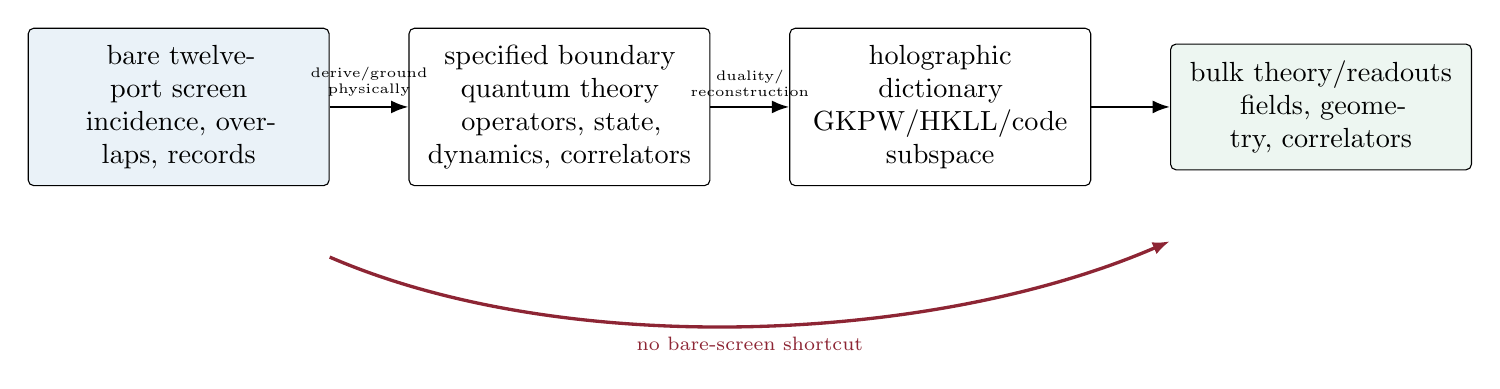
\begin{tikzpicture}[node distance=11mm and 10mm,
  box/.style={draw,rounded corners=2pt,align=center,inner sep=6pt,text width=34mm,minimum height=14mm},
  arr/.style={-{Latex[length=2.2mm]},thick}]
\node[box,fill=LightBlue] (screen) {bare twelve-port screen\\incidence, overlaps, records};
\node[box,fill=white,right=of screen] (qft) {specified boundary quantum theory\\operators, state, dynamics, correlators};
\node[box,fill=white,right=of qft] (dict) {holographic dictionary\\GKPW/HKLL/code subspace};
\node[box,fill=LightGreen,right=of dict] (bulk) {bulk theory/readouts\\fields, geometry, correlators};
\draw[arr] (screen) -- node[above,font=\tiny,align=center]{derive/ground\\physically} (qft);
\draw[arr] (qft) -- node[above,font=\tiny,align=center]{duality/\\reconstruction} (dict);
\draw[arr] (dict) -- (bulk);
\draw[DeepRed,line width=1.2pt,-{Latex[length=2.2mm]}] ([yshift=-9mm]screen.south east) .. controls +(3,-1.3) and +(-3,-1.3) .. node[below,font=\scriptsize,text=DeepRed]{no bare-screen shortcut} ([yshift=-9mm]bulk.south west);
\end{tikzpicture}%
}
\caption{The holographic typing obstruction.  HKLL is downstream of a
specified boundary quantum theory and a reconstruction dictionary; it is not a
map from a finite incidence drawing directly to a physical bulk.}
\label{fig:holochain}
\end{figure}

\subsection{The same twelve-point carrier supports different physics}

The failure already occurs before holography.  Put twelve qubits on the same
icosahedral incidence graph \(K_{12}\), with
\[
\mathcal H=(\mathbb C^2)^{\otimes 12}.
\]
Consider two Hamiltonians on exactly that carrier:
\[
H_0=0,
\qquad
H_J=J\sum_{\langle ij\rangle\in E(K_{12})}Z_iZ_j,
\qquad J\neq0.
\]
The screen, port count, edge count and incidence are identical.  The dynamics,
spectra, time evolution and generic correlation functions are not.  Therefore
the forgetful map
\[
U:\mathsf{BoundaryTheory}\to\mathsf{BareScreen}
\]
has a non-singleton fibre over the same twelve-port screen.

\begin{theorem}[No boundary theory from bare screen]
\label{thm:noboundary}
If \(B_1\neq B_2\) and \(U(B_1)=U(B_2)\), then there is no selector
\(S:\mathsf{BareScreen}\to\mathsf{BoundaryTheory}\) satisfying
\(S(U(B))=B\) for every boundary theory \(B\).
\end{theorem}

\begin{proof}
If such \(S\) existed,
\[
B_1=S(U(B_1))=S(U(B_2))=B_2,
\]
contradicting \(B_1\neq B_2\).
\end{proof}

\begin{theorem}[No Bulk From Bare Boundary]
\label{thm:nobulk}
Let \(H:\mathsf{BoundaryTheory}\to\mathsf{BulkTheory}\) be any bulk
assignment/reconstruction on a class of boundary theories.  If
\[
U(B_1)=U(B_2)
\quad\text{but}\quad
H(B_1)\neq H(B_2),
\]
then no map \(\widehat H:\mathsf{BareScreen}\to\mathsf{BulkTheory}\) can
satisfy \(H=\widehat H\circ U\).
\end{theorem}

\begin{proof}
Factorization would give
\[
H(B_1)=\widehat H(U(B_1))=\widehat H(U(B_2))=H(B_2),
\]
a contradiction.
\end{proof}

The theorem is deliberately general.  It does not assert that every twelve-
site spin system has an AdS dual.  It establishes the logically prior fact
that a bare screen is insufficient even to select the boundary dynamics that
a reconstruction dictionary would consume.  Holography cannot repair missing
input data by vocabulary.

\subsection{Why HKLL sharpens rather than weakens the reductio}

HKLL reconstructs a local bulk field using boundary operators in a specified
AdS/CFT setting.  Schematically,
\[
\phi_{\rm bulk}(X)
=\int_{\partial\mathrm{AdS}}K(X\mid x)\,\mathcal O(x)\,dx .
\]
The boundary operator \(\mathcal O\), its state/correlators and the smearing
kernel are not determined by the statement ``there are twelve points.''  The
kernel is tied to bulk/boundary dynamics and geometry; the boundary operators
belong to a specified quantum theory~\cite{HKLL2006}.  In the quantum-error-
correcting formulation, bulk operators are logical information encoded in a
boundary code structure, again presupposing the code, state space and operator
algebra~\cite{ADH2015}.

The relevant distinction is therefore not ``real versus mathematical'' in a
naive sense.  Both sides of a duality are mathematical descriptions.  The
physical distinction is that the AdS/CFT dictionary relates already specified,
physically interpreted quantum/gravitational degrees of freedom within a
candidate physical duality.  A bare cartoon or incidence graph has no such
status merely because one calls it a holographic screen.

\section{Physical closure cannot be source-only}
\label{sec:closure}

It is useful to separate six logically different closure levels:
\begin{enumerate}[label=\textbf{C\arabic*.}]
\item \textbf{Formal consistency:} the source axioms have models.
\item \textbf{Source determination:} desired mathematical objects are unique
inside the source language.
\item \textbf{Physical instantiation:} the source represents an actually
realized physical system.
\item \textbf{Boundary-theory closure:} the relevant physical boundary
operator algebra, state and dynamics are fixed.
\item \textbf{Holographic closure:} a valid boundary-to-bulk dictionary/code
subspace is fixed and reconstructs the claimed bulk observables.
\item \textbf{Empirical closure:} reconstructed observables are calibrated to
and survive independent experiment.
\end{enumerate}

Source-internal theorem proving can move within C1--C2.  \Cref{thm:alchemy}
blocks a purely logical jump from C2 to C3.  \Cref{thm:noboundary} blocks a
bare-screen jump to C4.  \Cref{thm:nobulk} blocks a bare-screen shortcut to C5.
Experiment and calibration are required for C6.

\begin{noescape}[Source-only physical-closure impossibility]
\label{thm:closure-impossible}
Let \(T_S\) be any satisfiable source theory whose extensions remain entirely
source-internal.  Suppose physical closure requires (i) nonempty external
physical realization, (ii) a physically specified boundary theory, and (iii)
a bulk reconstruction whose physical readouts are unique.  Then no sequence
of source-only enrichments of \(T_S\) can establish physical closure.  A
successful closure must introduce independently grounded physical structure
at or before the realization/boundary-theory stage.
\end{noescape}

The theorem gives an exhaustive dichotomy for a programme such as OPH:
\[
\boxed{
\begin{array}{ll}
\text{Remain source-only} & \Longrightarrow\ \text{physical closure is impossible},\\[1.5mm]
\text{add physical boundary/dictionary structure} & \Longrightarrow\ \text{closure is not from A1--A3 alone}.
\end{array}}
\]
There is no theorem-count escape.  More source consequences can characterize
the formal screen with increasing precision, but they cannot create the
external realization relation or supply a missing boundary quantum theory.

\section{Version lock and target of the audit}
\label{sec:versionlock}

\subsection{Frozen OPH basis}

The public target is the OPH repository at commit
\begin{center}
\texttt{40b13bb4bc56261f84fd515701916c388c42fe83},
\end{center}
committed on 26 August 2026.  The reader-facing normative basis is
\texttt{docs/AXIOM\_REFERENCE.md}; the repository also names a machine-readable
axiom registry.  At this commit OPH declares three core axioms:

\begin{enumerate}[label=\textbf{A\arabic*.}]
\item an oriented twelve-port observer-screen architecture with a finite
carrier federation, seams, records, readback, repair interfaces, an
icosahedral boundary packet, an \(S^2\) refinement support and a finite compact
unitary response algebra;
\item natural agreement of accepted observer-accessible data and operational
meaning across overlaps, rechartings, transports and refinements;
\item a conditional maximum-randomness/information-projection rule selecting a
state inside a fixed feasible family relative to declared reference data.
\end{enumerate}

The same reference expressly separates these source axioms from laboratory
identification, global compact-group selection, field lists, multiplicities,
model-space selection, couplings and other physical attachments.  It also
states that an exact result inside one named realization does not establish
that the axioms select that realization~\cite{OPHAxiomReference}.

\subsection{Live public-claim snapshot}

The logical theorems below are version-independent, but the current public
claim surface remains relevant.  At the frozen main-branch snapshot
\texttt{05207466cf63461c683bf1b8543d7c4a5feea4fa}, OPH describes itself as a
zero-dial theory-of-everything programme in which observers are primary,
objective reality is emergent, and overlap repair on a holographic screen is
used as the route toward quantum theory, spacetime, gravity, gauge structure,
matter and constants~\cite{OPHCurrentREADME}.  The same README advertises more
than 8800 Lean theorems while also acknowledging that the physical attachment
of its fixed-point closure remains open.  This juxtaposition is exactly what
the present theorem separates: source-proof volume and physical establishment
are different quantities.

An archived explanatory chapter is even more explicit about the intended
holographic move: it contrasts AdS/CFT's specific boundary CFT with an OPH
observer-horizon programme in which no global boundary CFT is required and the
bulk is said to emerge from agreement/consistency of overlapping observer
cuts~\cite{OPHArchivedHolography}.  That text is historical rather than the
normative axiom registry; it is cited only to identify the physical intuition
that \cref{sec:nobulk} audits.

\subsection{Claim under audit}

The theorem does not require OPH to make one exact sentence in every public
surface.  It audits the following general claim schema:
\begin{equation}
\label{eq:claim-schema}
\text{A1--A3 and their source consequences uniquely recover physical structure }C.
\end{equation}
Here \(C\) may be a physical gauge interaction, matter content, gravity,
spacetime, coupling, measured constant, particle spectrum, laboratory current
or any other experimentally meaningful object.

If OPH labels a result only as a conditional interface, named realization or
physical identification, the no-go does not contradict that narrower status.
It instead proves why the narrower status is required.  The result directly
blocks only the stronger wording in \cref{eq:claim-schema} unless a unique
realization theorem is supplied.

\subsection{Why version locking is non-negotiable}

A rapidly changing theory can answer a countermodel by adding premises.  That
may improve the new theory, but it cannot alter what followed from the earlier
one.  We therefore write \(T_h\) for the theory at repository hash \(h\).
Every entailment statement below has the form
\[
T_h\models C
\qquad\text{or}\qquad
T_h\notmodels C.
\]
A later \(T_{h'}=T_h\cup\Delta\) is audited separately.  This prevents a new
premise from being presented retroactively as an old theorem.

\section{Formal setting}
\label{sec:formalsetting}

\subsection{Source and physical languages}

Let \(\Lsrc\) be a signature containing exactly the source objects and maps of
a theory.  For the OPH application these include the frozen A1--A3 objects:
patches, ports, incidence, algebras, records, restriction maps, accepted
updates, response representations, interpretation functors, feasible states,
reference families and the information-projection rule.

Let \(\Lphys\supseteq\Lsrc\) extend the source language by physical objects
needed to express empirical claims.  Depending on the branch, these may
include:
\[
\begin{gathered}
\text{spacetime events and metrics, Hamiltonians, stress-energy, fields,}\\
\text{global gauge groups, matter representations, couplings, detector maps,}\\
\text{scattering amplitudes, spectra, clocks and laboratory records.}
\end{gathered}
\]
A physical model \(P\) has a source reduct
\[
U(P)=P\restr\Lsrc,
\]
obtained by forgetting the additional physical structure.  In model-theoretic
language, \(P\) is an \(\Lphys\)-expansion of \(U(P)\).  Categorically, \(U\)
is a forgetful functor
\[
U:\Phys\longrightarrow\Src.
\]

\begin{definition}[Realization fibre]
For a source model \(M\in\Src\), the realization fibre is
\[
\Real(M)=U^{-1}(M),
\]
the class or category of admissible physical expansions whose source reduct is
\(M\).
\end{definition}

\subsection{Physical equivalence}

Let \(\Obs\) be the declared family of physical readouts.  Each
\(O\in\Obs\) maps a physical model to a calibrated outcome in an outcome
space \(Y_O\).

\begin{definition}[Observational equivalence]
\[
P\obsim Q
\quad\Longleftrightarrow\quad
\forall O\in\Obs,\;O(P)=O(Q).
\]
\end{definition}

This is deliberately stronger than identity of source-language answers.  A
physical distinction is active when at least one admitted physical readout
separates the models.

\begin{definition}[Physical determination]
The source theory physically determines its realization relative to \(\Obs\)
when every realization fibre is observationally singleton:
\[
\forall M\models\Tsrc,\quad
\forall P,Q\in\Real(M),\quad P\obsim Q.
\]
\end{definition}

This definition allows many mathematical presentations of the same physics.
It asks only that the source determine one observational equivalence class.
It therefore cannot be defeated by harmless notation changes, coordinate
changes or genuine gauge redundancy.

\subsection{Gauge equivalence}

Let \(P\gaugesim Q\) denote gauge equivalence.  The defining physical
requirement is
\begin{equation}
\label{eq:gauge-preserves}
P\gaugesim Q\quad\Longrightarrow\quad P\obsim Q.
\end{equation}
If a readout is gauge invariant and differs, the two models are not related by
gauge.  This simple condition closes the claim that a counterexample is merely
a redescription.

\section{Borrowed machinery}

\subsection{Reducts and expansions}

If two \(\Lphys\)-structures have the same \(\Lsrc\)-reduct, every
\(\Lsrc\)-sentence has the same truth value in both.  This is not a new
physical principle.  It is the definition of reduct and satisfaction.  It
means that no amount of proof performed solely in \(\Lsrc\) can distinguish
the two expansions.

\subsection{Implicit and explicit definability}

A new physical relation \(R\) is \emph{implicitly definable} by \(\Tsrc\) if
no two models of the extended theory can agree on the entire source reduct and
disagree on \(R\).  In first-order logic, Beth's definability theorem says
that implicit definability entails explicit definability: there exists a
source-language formula \(\varphi_R\) such that
\[
R(\bm x)\longleftrightarrow\varphi_R(\bm x)
\]
in every model of the theory~\cite{Beth1953,Hodges1993}.

Beth's theorem is used here as a demand, not as the sole proof.  If a proponent
claims that physical meaning is uniquely ``implicit'' in the source
architecture, then in the first-order regime an explicit definition should
exist.  If the formalism is higher-order or categorical, the direct
realization-fibre theorem below still applies without Beth.

\subsection{Information projection}

An information projection has the form
\[
\rho_*\in\arg\min_{\rho\in\mathcal K}
D(\rho\Vert\tau),
\]
where \(\mathcal K\) is a fixed feasible set and \(\tau\) a fixed reference
state.  Standard \(I\)-projection theory studies existence, uniqueness and
geometry inside that declared space~\cite{KullbackLeibler,Csiszar1975}.  It
does not, without further structure, select among different field lists,
spacetimes, Hamiltonians or ontology classes.  The distinction is the familiar
one between state inference within a model and model-class identification.

\subsection{Categorical form}

The model-theoretic condition has a direct categorical translation.  The
source determines physical reality exactly when every fibre of
\(U:\Phys\to\Src\) is contractible after quotienting by observational
equivalence.  A fibre containing two observationally separated objects is not
contractible.  Adding more arrows or theorems inside the base category
\(\Src\) does not remove that multiplicity; one must constrain the lift.

\section{The ten-theorem no-wiggle suite}
\label{sec:theorems}

\subsection{T1: versioned entailment}

\begin{theorem}[Version-lock theorem]
Let \(T_h\) be the theory determined by a frozen signature, axiom set and
repository hash \(h\).  Whether \(T_h\models C\) is independent of premises
added only in a later theory \(T_{h'}=T_h\cup\Delta\).
\end{theorem}

\begin{proof}
Entailment from \(T_h\) is quantified over models of \(T_h\).  Restricting to
the smaller class of models satisfying \(\Delta\) may make \(C\) true in
\(T_{h'}\), but it does not remove countermodels of \(T_h\) from the historical
model class of \(T_h\).  Hence a later proof from \(T_{h'}\) is not a proof
from \(T_h\).
\end{proof}

\subsection{T2: source-language indiscernibility}

\begin{lemma}[Reduct indiscernibility]
If
\[
P\restr\Lsrc\cong Q\restr\Lsrc,
\]
then every source-language sentence \(\sigma\) has the same truth value in
\(P\) and \(Q\).
\end{lemma}

\begin{proof}
Satisfaction of an \(\Lsrc\)-sentence depends only on the interpretation of
symbols in \(\Lsrc\).  Isomorphic reducts preserve satisfaction.
\end{proof}

\begin{resultbox}[Consequence]
A proof assistant can certify arbitrarily many \(\Lsrc\)-theorems without
selecting between \(P\) and \(Q\).  The issue is not proof quantity; it is
whether the physical lift is determined.
\end{resultbox}

\subsection{T3: two-expansion non-uniqueness}

\begin{theorem}[Two-expansion theorem]
\label{thm:two-expansion}
Let \(M\models\Tsrc\).  If \(P,Q\in\Real(M)\) and
\(P\not\obsim Q\), then \(\Tsrc\) does not physically determine its
realization.
\end{theorem}

\begin{proof}
Physical determination requires every pair in \(\Real(M)\) to be
observationally equivalent.  The pair \(P,Q\) violates that universal
condition.
\end{proof}

\begin{figure}[htbp]
\centering
\resizebox{\textwidth}{!}{%
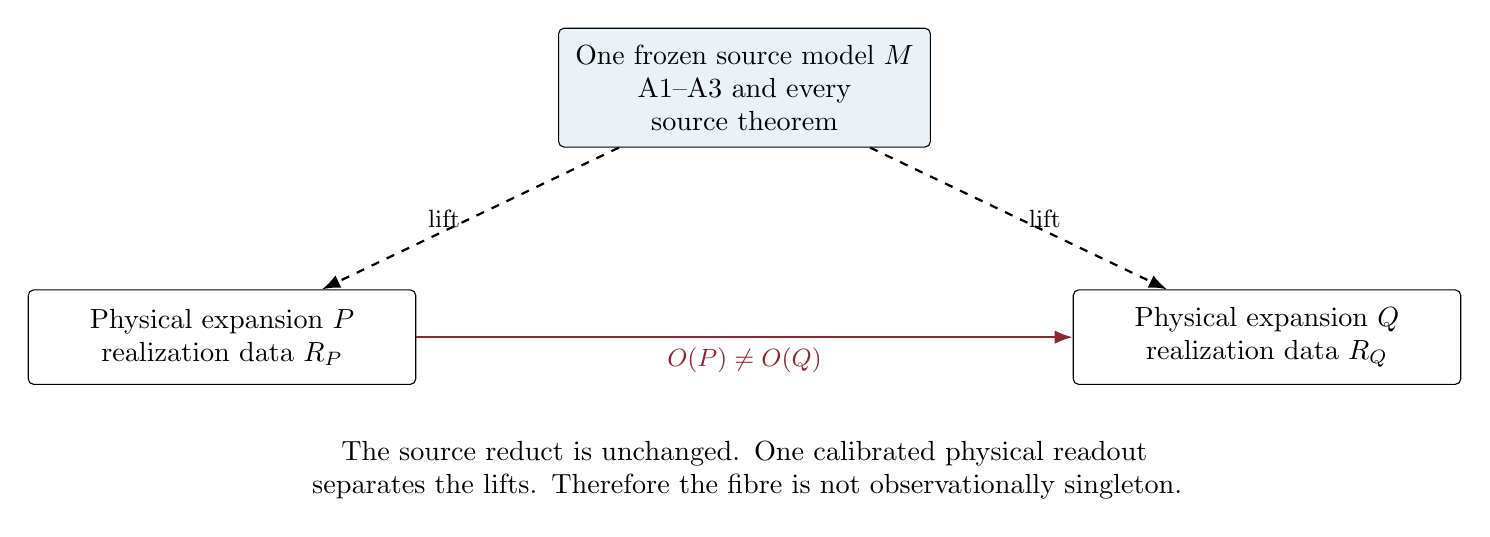
\begin{tikzpicture}[
  box/.style={draw,rounded corners=2pt,align=center,inner sep=6pt,minimum height=12mm},
  arr/.style={-{Latex[length=2.3mm]},thick},
  darr/.style={-{Latex[length=2.3mm]},thick,dashed}
]
\node[box,fill=LightBlue,text width=43mm] (M) {One frozen source model \(M\)\\A1--A3 and every source theorem};
\node[box,fill=white,text width=45mm,below left=18mm and 18mm of M] (P) {Physical expansion \(P\)\\realization data \(R_P\)};
\node[box,fill=white,text width=45mm,below right=18mm and 18mm of M] (Q) {Physical expansion \(Q\)\\realization data \(R_Q\)};
\draw[darr] (M) -- node[left,font=\small]{lift} (P);
\draw[darr] (M) -- node[right,font=\small]{lift} (Q);
\draw[arr,DeepRed] (P) -- node[below,font=\small,text=DeepRed]{\(O(P)\neq O(Q)\)} (Q);
\node[align=center,text width=115mm,below=12mm of $(P)!0.5!(Q)$] {The source reduct is unchanged.  One calibrated physical readout separates the lifts.  Therefore the fibre is not observationally singleton.};
\end{tikzpicture}%
}
\caption{The universal counterexample pattern.  It is invariant under changes
of notation and does not challenge source-internal theorem validity.}
\label{fig:fibre}
\end{figure}

\subsection{T4: observable separation}

\begin{theorem}[Observable-witness theorem]
If there exists \(O\in\Obs\) for which \(O(P)\neq O(Q)\), then
\(P\not\obsim Q\).
\end{theorem}

\begin{proof}
Observational equivalence requires equality for every member of \(\Obs\).
One counterexample readout negates the universal statement.
\end{proof}

This apparently trivial theorem is load bearing.  It prevents a response from
moving the disagreement into an undefined metaphysical category.  The witness
is a physical record: a cross section, spectrum, clock comparison, current,
Wilson line, detector count, lensing map or other calibrated outcome.

\subsection{T5: no gauge escape}

\begin{theorem}[Gauge-escape no-go]
Assume gauge equivalence preserves every admitted readout as in
\cref{eq:gauge-preserves}.  If \(O(P)\neq O(Q)\) for a gauge-invariant
\(O\), then \(P\not\gaugesim Q\).
\end{theorem}

\begin{proof}
If \(P\gaugesim Q\), \cref{eq:gauge-preserves} gives \(O(P)=O(Q)\),
contradicting the witness.
\end{proof}

Thus the counterexample must be answered physically, not by calling the two
models different presentations.

\subsection{T6: Beth's explicit-definition demand}

\begin{corollary}[Beth fork]
\label{cor:bethfork}
In a first-order formalization, a physical relation that is uniquely implicitly
determined by \(\Tsrc\) must be explicitly definable in \(\Lsrc\).  Therefore
one of the following holds:
\begin{enumerate}[label=(\roman*)]
\item an explicit source-language definition is supplied;
\item the relation is additional primitive structure;
\item unique determination fails.
\end{enumerate}
\end{corollary}

\begin{proof}
Beth's definability theorem gives (i) whenever implicit definability genuinely
holds.  If no such definition is part of the theory and the physical relation
is nevertheless included, it is primitive, giving (ii).  Otherwise there are
models agreeing on the source reduct and differing on the relation, giving
(iii).
\end{proof}

The corollary blocks the phrase ``the physical meaning is implicit'' from
serving as a proof.  Implicit uniqueness is itself a mathematical claim with a
definability consequence.

\subsection{T7: information-projection blindness}

\begin{theorem}[Source-blind optimization theorem]
\label{thm:iprojection}
Let \(U:\Phys\to\Src\) be the source reduct.  Suppose the feasible predicate
and objective factor through \(U\):
\[
K(P)=K_0(U(P)),
\qquad
J(P)=J_0(U(P)).
\]
If \(U(P)=U(Q)\), then
\[
K(P)\Longleftrightarrow K(Q),
\qquad
J(P)=J(Q).
\]
Consequently, a minimization rule using only \(K\) and \(J\) cannot uniquely
select one of two distinct same-reduct lifts.
\end{theorem}

\begin{proof}
Factorization gives
\[
K(P)=K_0(U(P))=K_0(U(Q))=K(Q)
\]
and the identical calculation for \(J\).  If \(P\) is feasible and minimizes
\(J\), then \(Q\) is feasible with the same objective value and is also a
minimizer.  Uniqueness fails unless the rule uses information not factoring
through the source reduct.
\end{proof}

\begin{resultbox}[Application to maximum randomness]
A3 may uniquely select a state in a fixed OPH source feasible space.  It cannot
select a unique Hamiltonian, field list, physical interpretation, global gauge
form or laboratory map when those structures are absent from that source
space.  Adding them to the feasible space or reference measure makes them
inputs to the selection problem.
\end{resultbox}

\subsection{T8: the interpretation-functor fork}

\begin{theorem}[Interpretation-functor theorem]
\label{thm:interpretationfork}
Let a source model contain an interpretation map
\(\mathcal J:\mathsf{Data}\to\mathsf{Meaning}\).  For a physical
identification encoded through \(\mathcal J\), at least one of the following
holds:
\begin{enumerate}[label=(\alph*)]
\item \(\mathcal J\) is fixed with the required empirical semantics, in which
case that semantics is source data;
\item multiple admissible \(\mathcal J\)'s survive, in which case physical
meaning is underdetermined;
\item \(\mathcal J\) is uniquely constructed from earlier source structure,
in which case the construction and uniqueness theorem must be displayed.
\end{enumerate}
\end{theorem}

\begin{proof}
Either the map is primitive in the model specification, allowed to vary over a
class of models, or determined by the remaining structure.  These cases are
exhaustive.  In the first, its physical content is assumed; in the second,
there are distinct expansions; in the third, uniqueness is a theorem
obligation.  Naturality constrains a chosen \(\mathcal J\) but does not by
itself choose its codomain semantics or select one functor among all natural
ones.
\end{proof}

This theorem is essential for observer-first languages.  The word ``meaning''
cannot make the source-to-physics map disappear.  If laboratory meaning is
already encoded in \(\mathcal J\), it has entered at the axiom.  If not, the
physical lift remains to be derived.

\subsection{T9: conservative-extension accounting}

\begin{theorem}[Added-premise accounting]
\label{thm:addedpremise}
If
\[
T_h\notmodels C
\qquad\text{but}\qquad
T_h\cup\Delta\models C,
\]
then \(\Delta\) is load bearing for \(C\).  The strongest accurate statement
is that \(C\) follows from \(T_h\cup\Delta\), not from \(T_h\).
\end{theorem}

\begin{proof}
The first relation supplies a model of \(T_h\) in which \(C\) fails.  Every
proof of \(C\) from the extended theory therefore excludes at least that model
through \(\Delta\).  Deleting \(\Delta\) restores the countermodel.
\end{proof}

If \(\Delta\) is an independently measured physical principle, the extended
theory may be scientifically sound.  But zero-input, three-axiom or pure
source-recovery language must be withdrawn.  If \(\Delta\) merely says to
select the observed target, it is circular.

\subsection{T10: downstream non-determination}

\begin{theorem}[Downstream collapse schema]
\label{thm:downstream}
Let \(F\) be any physical feature or downstream observable.  If there exist
\(P,Q\) with
\[
U(P)=U(Q)
\qquad\text{and}\qquad
F(P)\neq F(Q),
\]
then \(\Tsrc\) does not determine \(F\).
\end{theorem}

\begin{proof}
Determination of \(F\) requires \(F\) to be constant on every realization
fibre.  The witness pair shows it is not constant on \(\Real(U(P))\).
\end{proof}

This is how one countermodel can govern thousands of downstream lemmas.  Any
internal theorem whose conclusion is entirely source-algebraic may remain
valid.  Every physical conclusion that changes across the witness pair is not
a consequence of the shared source theory.

\section{The master no-escape trilemma}

\begin{noescape}[Physical realization trilemma]
\label{thm:master}
For a version-locked source theory \(T_h\) and a claimed uniquely recovered
physical structure \(C\), at least one of the following is true:
\begin{enumerate}[label=\textbf{\Roman*.}]
\item \textbf{Explicit derivation.}  A source-language definition or unique,
functorial realization construction is supplied and proved to preserve all
admitted physical readouts.
\item \textbf{Additional physical structure.}  A realization map, physical
selector, empirical attachment or equivalent premise is added beyond the
neutral source theory.
\item \textbf{Failure or restricted scope.}  Two observationally inequivalent
physical expansions share the same source reduct, so unique physical recovery
fails; alternatively the separating readout is excluded, in which case the
theory does not recover that physical domain.
\end{enumerate}
No change of terminology, relabelling, gauge language, entropy maximization or
later axiom addition produces a fourth possibility.
\end{noescape}

\begin{proof}
If the physical structure is uniquely determined in the first-order regime,
\cref{cor:bethfork} demands an explicit definition; in the general categorical
regime, every realization fibre must be observationally singleton.  This is
case I.  If the selector is instead present as primitive interpretation or an
added interface, case II holds by \cref{thm:interpretationfork,thm:addedpremise}.
If neither is true, the physical relation is not fixed by the source; a
same-reduct pair can differ on it, and any admitted separating readout invokes
\cref{thm:two-expansion}.  If the readout is declared inadmissible, the theory
has restricted its physical scope.  Relabellings preserve reduct isomorphism;
gauge transformations preserve readouts; source-factorized entropy cannot
separate lifts by \cref{thm:iprojection}; later additions are counted by
\cref{thm:addedpremise}.  The cases exhaust the logical possibilities.
\end{proof}

\begin{figure}[htbp]
\centering
\resizebox{\textwidth}{!}{%
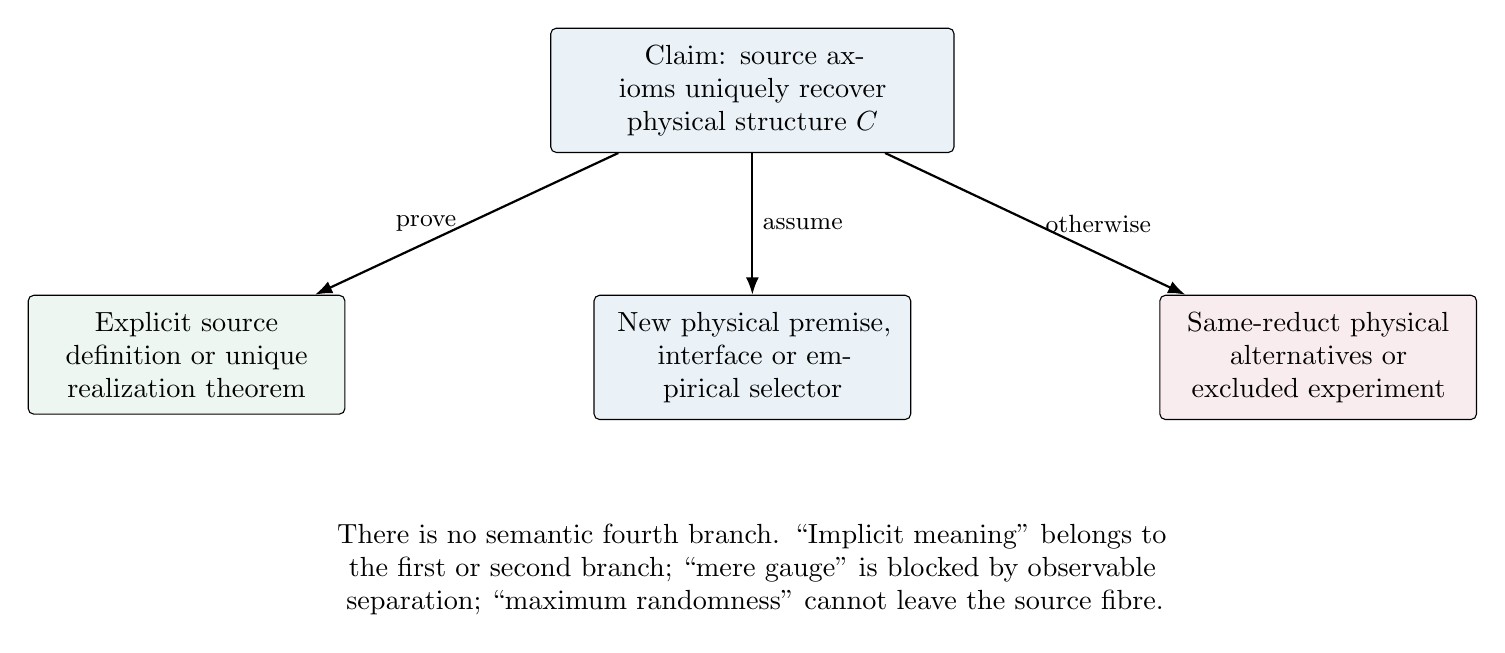
\begin{tikzpicture}[
  node distance=12mm and 11mm,
  box/.style={draw,rounded corners=2pt,align=center,inner sep=6pt,text width=36mm,minimum height=15mm},
  arr/.style={-{Latex[length=2.2mm]},thick}
]
\node[box,fill=LightBlue,text width=47mm] (claim) {Claim: source axioms uniquely recover physical structure \(C\)};
\node[box,fill=LightGreen,below left=18mm and 26mm of claim] (derive) {Explicit source definition or unique realization theorem};
\node[box,fill=LightBlue,below=18mm of claim] (add) {New physical premise, interface or empirical selector};
\node[box,fill=LightRed,below right=18mm and 26mm of claim] (fail) {Same-reduct physical alternatives or excluded experiment};
\draw[arr] (claim) -- node[left,font=\small]{prove} (derive);
\draw[arr] (claim) -- node[right,font=\small]{assume} (add);
\draw[arr] (claim) -- node[right,font=\small]{otherwise} (fail);
\node[align=center,text width=155mm,below=12mm of add] {There is no semantic fourth branch.  ``Implicit meaning'' belongs to the first or second branch; ``mere gauge'' is blocked by observable separation; ``maximum randomness'' cannot leave the source fibre.};
\end{tikzpicture}%
}
\caption{The exhaustive no-escape trilemma.}
\label{fig:trilemma}
\end{figure}

\section{Application to the frozen OPH basis}
\label{sec:application}

\subsection{What A1--A3 actually fix}

The Mr Tickle reductio applies only to what the source language actually
protects.  It does not require changing A1's abstract icosahedral packet.  One
keeps the same packet, algebras, records, overlaps, response and refinement
maps and changes only the pictorial/presentational carrier.  OPH's own A1
reference explicitly treats embedding coordinates, materials and hidden
presentation details as non-protected while retaining the abstract incidence
and operational maps~\cite{OPHAxiomReference}.  Therefore appearance cannot
be the missing physical selector.  If the source model is physically promoted,
the promotion must come from something other than the fact that one drawing
looks more scientific than another.


At the frozen commit, OPH's A1 fixes a highly structured mathematical source:
an oriented twelve-port carrier boundary, a federation and overlap nerve, an
\(S^2\) support tower, central record algebras, restriction and update
interfaces, and a faithful finite compact response algebra.  A2 imposes
naturality and internal implementation of accepted rechartings.  A3 chooses an
information projection on a fixed accessible algebra and fixed feasible
family~\cite{OPHAxiomReference}.

This is substantial mathematics.  It is also not yet a unique physical world.
The axiom reference itself states, in substance, that:

\begin{itemize}
\item A1 does not select laboratory identification, a particular global
compact group, particles or couplings;
\item A2 does not select a global compact group or laboratory interpretation;
\item A3 selects a state inside one fixed model space and cannot compare
unrelated field lists, Hilbert spaces or ontology classes without a common
source space;
\item later gravity, gauge, matter, flavour and quantitative conclusions must
display the additional structure they consume;
\item a named-realization witness proves existence inside that realization,
not selection by the axioms.
\end{itemize}

These scope clauses are consistent with the theorem in this paper.  They also
mean that any public claim that A1--A3 alone uniquely recover the complete
physical universe overstates the frozen formal basis.

\subsection{The featureless source witness}

The 2 August countermodel constructed an abstract oriented icosahedral carrier
with twelve ports, a twelve-dimensional compact response algebra, internal
\(A_5\) action, functorial agreement and a maximum-randomness state.  It
recovered the conditional Lie-algebra type
\[
\mathfrak u(1)\oplus\mathfrak{su}(2)\oplus\mathfrak{su}(3)
\]
without giving any object a physical interpretation~\cite{AnonFeatureless}.
The result established the earlier branch-specific theorem:
\[
\text{source algebraic recovery}
\not\Longrightarrow
\text{physical Standard Model realization}.
\]

OPH has since strengthened and expanded A1--A3.  The present article therefore
does not depend on every detail of the old finite witness satisfying every new
clause.  Instead it applies the universal fibre theorem to any source model
that OPH itself accepts at the frozen commit.  If no model satisfies the
strengthened axioms, the source theory has no realization.  If at least one
model \(M\) does, the physical-lift question is governed by
\cref{thm:master}.

\subsection{A bona fide physical pair: coupling freedom}

To prevent the objection that one branch is ``merely nonphysical'', consider
two ordinary physical quantum field theories built over the same recovered
local response algebra.  Use the \(\mathfrak u(1)\) factor and fix the same
matter content, spacetime, masses, states and detector definitions.  For each
positive coupling \(e\), define
\begin{equation}
\label{eq:qed}
\mathcal L_e
=
-\frac14 F_{\mu\nu}F^{\mu\nu}
+\bar\psi(i\gamma^\mu\partial_\mu-m)\psi
-e\,\bar\psi\gamma^\mu A_\mu\psi.
\end{equation}
The source reduct remembers the abstract \(\mathfrak u(1)\) response direction
and all OPH source structure, but not the physical coupling unless a coupling
selector has been added.  Hence for \(e\neq e'\),
\[
U(P_e)=U(P_{e'}).
\]
At tree level, a one-photon-exchange amplitude between charged matter states is
proportional to \(e^2\), and its differential cross section is generically
proportional to \(e^4\).  At fixed non-singular kinematics,
\[
\frac{d\sigma_e}{d\Omega}\neq
\frac{d\sigma_{e'}}{d\Omega}.
\]
The cross section is a calibrated, gauge-invariant physical record.  Therefore
\[
P_e\not\obsim P_{e'}.
\]
By \cref{thm:two-expansion}, A1--A3 do not determine the physical coupling.

There are only two replies.  OPH may add a unique coupling construction, in
which case that construction is a new load-bearing bridge and must be audited.
Or it may accept that the source algebra determines at most a response type,
not the measured interaction strength.

\subsection{A second physical pair: global gauge form}

A local Lie algebra does not by itself fix the global gauge theory.  Distinct
global forms and line-operator spectra can define physically distinct
four-dimensional gauge theories while sharing local algebraic data
\cite{AharonySeibergTachikawa}.  Thus even after recovering
\(\mathfrak u(1)\oplus\mathfrak{su}(2)\oplus\mathfrak{su}(3)\), a global
quotient, admissible line operators, matter representations and charge lattice
remain separate selection obligations.  If OPH derives these from additional
carrier and matter premises, those premises belong in the target theorem.  A
local-algebra proof alone cannot carry the global physical conclusion.

\subsection{A3 cannot choose between these lifts}

The OPH A3 objective is evaluated on the fixed source state family.  If
\(P_e\) and \(P_{e'}\) have the same source reduct, both the feasible source
state and the source-relative entropy objective are equal.  By
\cref{thm:iprojection}, A3 cannot prefer \(e\) to \(e'\).  A reference state or
constraint depending on \(e\) would solve a different problem in which the
coupling has already entered the input.

\subsection{The observer-language self-test}

OPH makes records and public agreement central.  That strengthens rather than
weakens the no-go.  If two physical lifts produce different stable public
records, an observer-based theory cannot identify them without either deleting
one admitted record or changing the source doctrine.  If the theory excludes
the scattering record in the coupling example, it does not recover the
physical domain in which that scattering experiment is performed.

\section{Exhaustive response classification}
\label{sec:responses}

\begin{longtable}{>{\raggedright\arraybackslash}p{0.25\textwidth}>{\raggedright\arraybackslash}p{0.34\textwidth}>{\raggedright\arraybackslash}p{0.32\textwidth}}
\toprule
\textbf{Attempted response} & \textbf{Formal requirement} & \textbf{Unavoidable consequence}\\
\midrule
\endfirsthead
\toprule
\textbf{Attempted response} & \textbf{Formal requirement} & \textbf{Unavoidable consequence}\\
\midrule
\endhead
``The countermodel is not physical.'' & Give a source-derived predicate that accepts the intended physical model and rejects the witness. & The predicate is either a new physical premise or an explicit realization theorem.\\
\addlinespace
``Physicality is supplied by an interface.'' & Specify the interface and prove uniqueness/future-faithfulness. & If not source-definable, the interface is additional structure, not an A1--A3 theorem.\\
\addlinespace
``A3 maximum randomness selects it.'' & Show the feasible set or objective differs between the physical lifts without importing physical data. & If both factor through the source reduct they tie; if they do not, the selector contains extra physical information.\\
\addlinespace
``They are gauge equivalent.'' & Show every gauge-invariant readout agrees. & One differing cross section, spectrum, clock or detector count blocks the claim.\\
\addlinespace
``That readout is inadmissible.'' & Remove it from \(\Obs\). & The theory no longer recovers the experimental domain containing that readout.\\
\addlinespace
``The words were intended physically.'' & Encode the intended semantics as a definition or axiom. & A definition must be proved unique; an axiom assumes the physical content.\\
\addlinespace
``The meaning is implicit.'' & Establish implicit definability across all source models. & In first-order logic Beth yields an explicit definition; otherwise a same-reduct pair defeats uniqueness.\\
\addlinespace
``We reinterpret the source objects.'' & Supply an isomorphism or translation. & Isomorphic redescription preserves the counterexample; changing readouts or premises creates a new theory.\\
\addlinespace
``We added a stronger axiom.'' & Freeze the new theory at a new hash. & The added axiom is load bearing; the earlier theory remains non-entailing.\\
\addlinespace
``We never claimed uniqueness.'' & Restrict the claim to a conditional construction or named realization. & This accepts the paper's conclusion and preserves only the narrower result.\\
\addlinespace
``The Lean corpus proves the branch.'' & Identify the exact theorem whose premises uniquely fix the physical lift. & Proof volume inside the source language cannot distinguish same-reduct physical expansions.\\
\addlinespace
``The witness changes hidden implementation.'' & Demonstrate that hidden change is future-inactive for all physical readouts. & If a physical readout changes, it is not hidden redundancy; if none changes, the witness is not observationally distinct.\\
\bottomrule
\end{longtable}

\begin{warningbox}[No semantic escape]
Every reply must modify the source premises, modify the observation family, or
accept non-uniqueness.  Renaming one of these moves does not change its logical
status.
\end{warningbox}

\section{What the result refutes, preserves and requires}

\subsection{Preserved results}

The following may remain correct:

\begin{itemize}
\item finite icosahedral incidence theorems;
\item exact statements about a declared response representation;
\item compact-Lie-algebra classifications under their hypotheses;
\item naturality and overlap-consistency theorems;
\item existence or exactness inside a named finite realization;
\item information-projection theorems on a fixed feasible space;
\item formal Lean proofs of those statements.
\end{itemize}

The paper does not attack a theorem merely because its words resemble physical
nouns.  It asks what the theorem's formal premises entail.

\subsection{Refuted overclaim}

What fails is the unrestricted arrow
\[
\boxed{
\text{A1--A3 source structure}
\Longrightarrow
\text{one uniquely determined physical world}
}
\]
whenever the realization fibre contains observationally inequivalent lifts.
The failure propagates to every downstream physical quantity that differs
across those lifts by \cref{thm:downstream}.

\subsection{Requirements for a successful repair}

A successful physical recovery theorem must supply all of the following:

\begin{enumerate}
\item a version-locked source theory;
\item a precisely typed physical target category;
\item a realization functor or relation;
\item existence for every relevant source model;
\item uniqueness up to observational equivalence;
\item preservation of gauge-invariant physical readouts;
\item proof that no target information was inserted into the source grammar,
reference state, candidate menu or interpretation map;
\item independent empirical calibration where dimensions and couplings enter.
\end{enumerate}

This is not an impossible standard.  It is the exact content of the claim that
a source architecture recovers physics rather than merely representing it.


\section{Theorem-volume irrelevance: an exact quantitative result}
\label{sec:volume}

The no-go can be sharpened into a quantitative statement about proof volume.
Let \(\tau_1,\ldots,\tau_N\) be any finite family of propositions whose
semantics factor through the frozen source reduct \(U\).  Define the joint
source-theorem fingerprint
\[
F_N(X)
=
\bigl(\mathbf 1_{\tau_1(X)},\ldots,\mathbf 1_{\tau_N(X)}\bigr)
\in\{0,1\}^N .
\]
The family may contain theorems, checked lemmas, finite certificates, derived
identities or any other Boolean judgements whose truth depends only on
\(U(X)\).

\begin{theorem}[Theorem-fingerprint invariance]
\label{thm:fingerprint}
If \(U(P)=U(Q)\) and every \(\tau_i\) factors through \(U\), then for every
finite \(N\),
\[
\boxed{F_N(P)=F_N(Q).}
\]
Consequently no deterministic classifier whose only input is the complete
\(N\)-theorem fingerprint can distinguish \(P\) from \(Q\).
\end{theorem}

\begin{proof}
For each \(i\) there exists a source predicate \(\bar\tau_i\) such that
\(\tau_i=\bar\tau_i\circ U\).  Hence
\[
\tau_i(P)=\bar\tau_i(U(P))
=\bar\tau_i(U(Q))=\tau_i(Q)
\]
for every \(i\).  Equality holds coordinatewise, so the fingerprints are
identical.  Any post-processing map receives the same input on the two lifts
and therefore returns the same output.
\end{proof}

Define the physical discrimination count of the theorem family on a witness
pair by
\[
D_N(P,Q)
:=
\sum_{i=1}^N
\mathbf 1\!\left[\tau_i(P)\neq\tau_i(Q)\right].
\]
On a same-reduct pair, \cref{thm:fingerprint} gives
\[
\boxed{D_N(P,Q)=0}
\qquad\text{and, for }N>0,\qquad
\boxed{\delta_N:=D_N/N=0.}
\]
This is an exact zero, not a statement that the theorem family is merely
``large'' or ``redundant''.

\subsection{Information-theoretic form}

The same result has a standard Shannon interpretation~\cite{Shannon1948}.
Let a binary random variable \(L\) choose equiprobably between two
observationally inequivalent lifts \(P\) and \(Q\) with the same source
reduct, and let
\[
Y=F_N(L)
\]
be the full theorem fingerprint observed by an analyst.  Because
\(F_N(P)=F_N(Q)\), \(Y\) is constant with respect to \(L\).  Therefore
\[
\boxed{I(L;Y)=0\ \text{bits}},
\qquad
\boxed{H(L\mid Y)=H(L)=1\ \text{bit}}.
\]
Thus the entire source-theorem corpus supplies exactly zero information about
which of the two physical lifts is realized.  With \(k\) equiprobable,
observationally inequivalent lifts in one source fibre,
\[
I(L;Y)=0,
\qquad
H(L\mid Y)=\log_2 k .
\]
The unresolved physical information is independent of \(N\).

\begin{warningbox}[What ``zero'' means]
This result does \emph{not} say that the source theorems are mathematically
meaningless.  It says something narrower and exactly measurable: their joint
truth vector has zero discriminatory power for choosing among physically
inequivalent lifts that share the same source reduct.  A theorem can be
perfectly correct internally while contributing zero bits to the missing
source-to-physics selection problem.
\end{warningbox}

\subsection{Numerical instantiation for OPH}

OPH's public 25 August 2026 commit states that its automated ``theorem floors''
were raised to \(8400\)~\cite{OPHTheoremFloor}; the live README checked on
26 August advertises more than \(8800\) Lean theorems~\cite{OPHCurrentREADME}.
Running OPH's own
\texttt{tools/check\_lean\_theorem\_count.py} against the frozen checkout used
for this audit returns \(8449\) public \texttt{theorem}/\texttt{lemma}
declarations across 381 Lean source files; the exact output and counting-script
hash accompany this article in \texttt{OPH\_THEOREM\_COUNT\_AUDIT.txt}.

The count itself does not establish that all 8449 declarations are
source-internal.  Instead the corpus is partitioned by a mathematically sharp
criterion.  Let
\[
S=\{i:\tau_i\text{ factors through }U\},
\qquad
E=\{1,\ldots,8449\}\setminus S.
\]
Every declaration in \(S\) is blind on the same-reduct witness pair, so
\[
D_S(P,Q)=0,
\qquad
I(L;F_S)=0\ \text{bits}.
\]
This includes any 5000-, 8400-, or 8449-element family for which source
factorization is actually established.

Conversely, if a declaration \(\tau_j\) does distinguish the two physical
lifts,
\[
\tau_j(P)\neq\tau_j(Q),
\]
then \cref{thm:fingerprint} immediately implies that \(\tau_j\) cannot factor
through the common source reduct.  Its discriminating content therefore comes
from structure outside that reduct: an additional physical premise,
realization map, calibration, target attachment, or strengthened axiom.  It
may be a valid theorem, but it cannot simultaneously be cited as evidence that
the original common source structure alone selected the physical lift.

Thus the raw number 8449 has no standalone evidentiary force for unique
physical recovery.  Each declaration falls into one of two relevant bins:
\[
\boxed{\text{source-factorized}\Rightarrow 0\text{ lift-discrimination bits}}
\]
or
\[
\boxed{\text{lift-separating}\Rightarrow\text{ beyond-source structure is load bearing}.}
\]
There is no third category in which a theorem both depends only on the common
source reduct and nevertheless distinguishes two models that have that same
reduct.

\begin{theorem}[Theorem volume cannot repair physical non-definability]
\label{thm:volume}
Let \(P,Q\) share a source reduct and be separated by an admitted physical
readout.  Adjoining any finite family of source-language theorems leaves both
facts unchanged:
\[
F_N(P)=F_N(Q)
\quad\text{and}\quad
P\not\sim_{\rm obs}Q.
\]
Hence no finite increase in source-internal theorem count can convert the
non-singleton realization fibre into a unique physical recovery.
\end{theorem}

This result isolates the only scientifically relevant escape.  A new result
must make a physical distinction that the old source reduct did not make.
Then it is either (i) an explicit derivation of additional physical structure
from stronger premises, or (ii) an additional physical premise/identification.
It cannot be credited retroactively to theorem volume already blind to that
distinction.



\section{Architectural convergence as a role-graph problem}
\label{sec:convergence}

The conceptual-ancestry question cannot be evaluated by counting shared words.
The relevant object is a dependency architecture.  Let
\[
G_P=(V_P,E_P,w)
\]
be the role graph extracted from a dated prior corpus, where vertices are
functional obligations---realization gate, record closure, dynamics before
action, admissible history before minimization, countermodel uniqueness,
premise ancestry, no-privilege selection, observer-history retention and
physical calibration---and edges record their logical order.  Let
\(x_t(v)\in[0,1]\) be the auditor-coded visibility of role \(v\) in a
version-locked OPH snapshot at time \(t\).

For role weights \(w_v\) and probative factors \(p_v\), define
\[
C_V(t)=\frac{\sum_v w_vp_vx_t(v)}{\sum_v w_vp_v}.
\]
For a directed edge \(e=(u,v)\), define
\[
x_t(e)=\min\{x_t(u),x_t(v)\},\qquad
C_E(t)=\frac{\sum_e w_ep_ex_t(e)}{\sum_e w_ep_e},
\quad p_e=\min\{p_u,p_v\}.
\]
These quantities are not probabilities of copying.  They are transparent
arithmetic conditional on a published coding table.  Every role, factor,
weight, snapshot value and evidence group is supplied in machine-readable
form so that a critic can change one entry and recompute the result.

\begin{figure}[htbp]
\centering
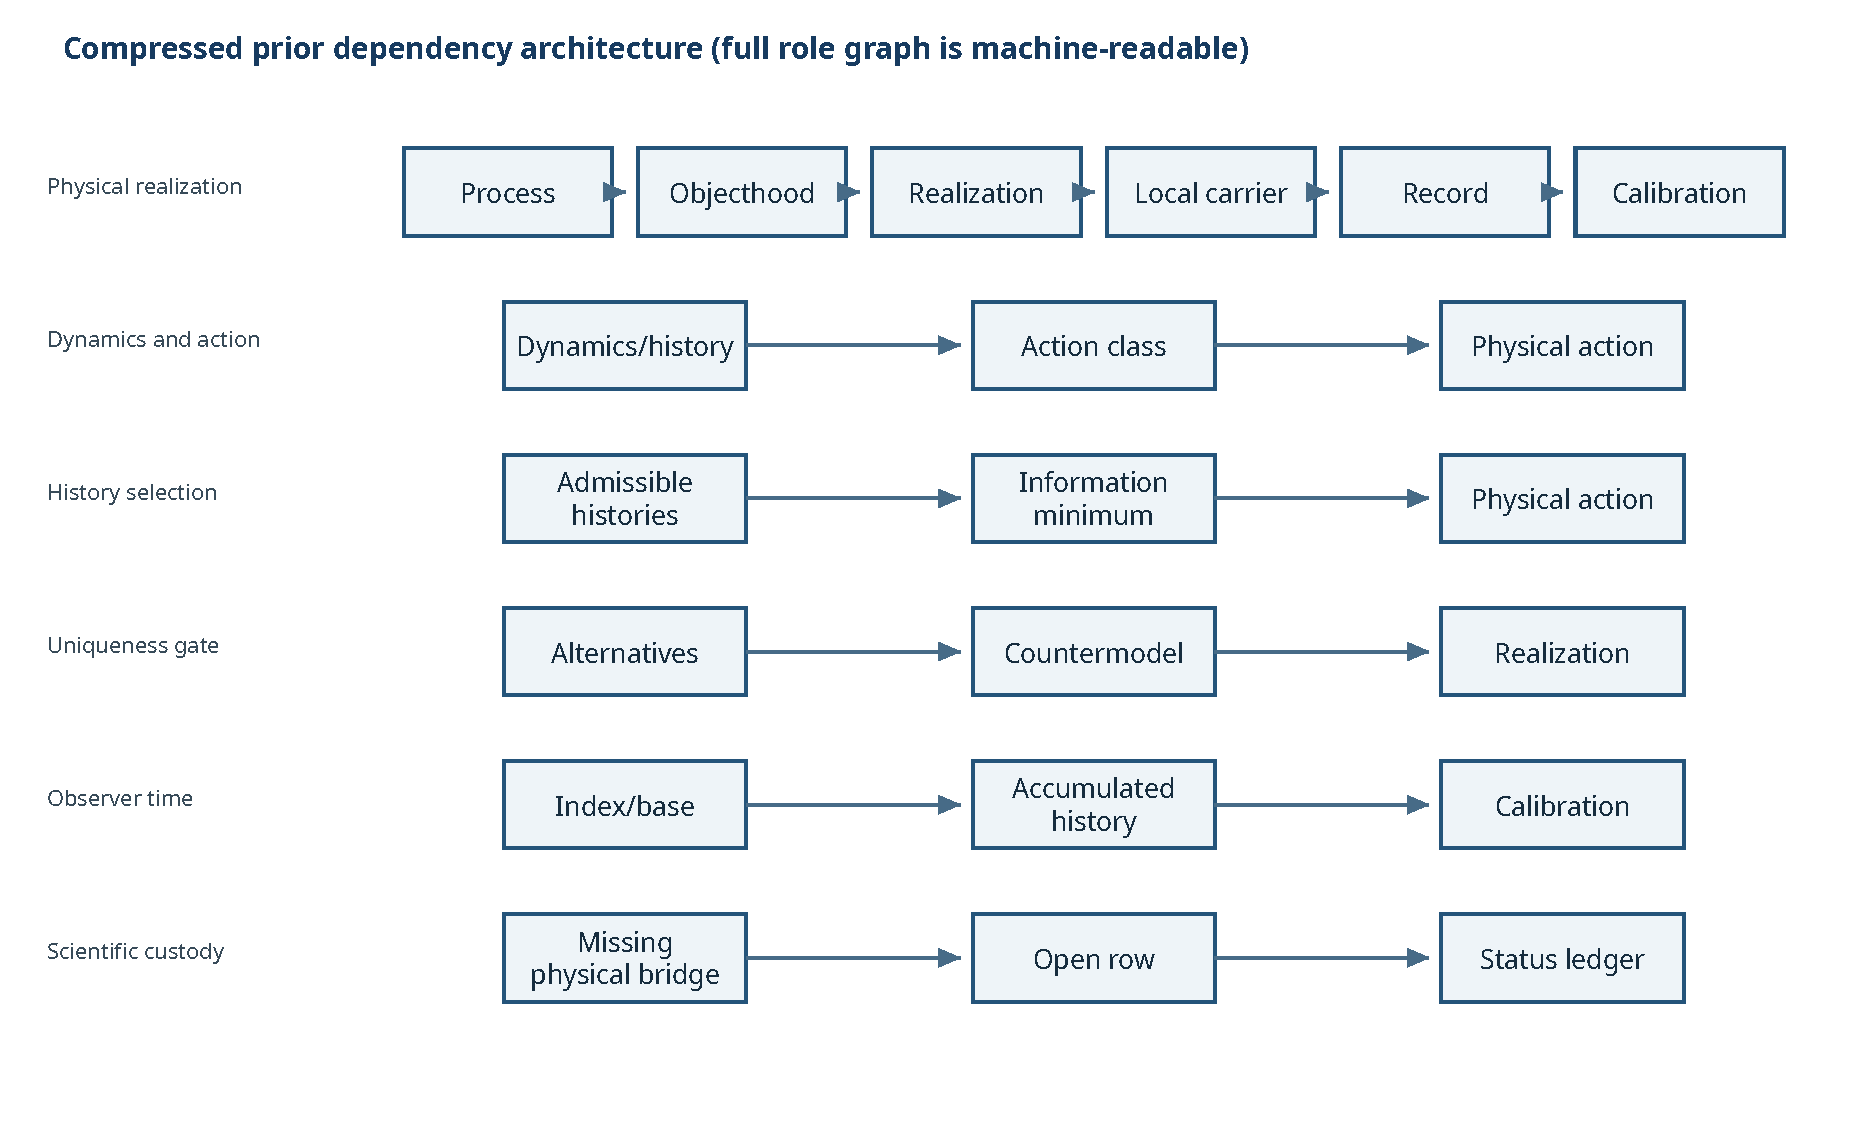
\includegraphics[width=0.98\textwidth]{../figures/prior_dependency_role_graph.pdf}
\caption{Compressed view of the prior functional dependency architecture.
The complete weighted role graph is distributed as JSON/DOT/SVG.  Nodes are
scientific functions rather than vocabulary; generic Born, Lorentz and
ordinary icosahedral/golden structures are controls.}
\label{fig:rolegraph}
\end{figure}

\subsection{Frozen coding, robustness and negative controls}

The coding down-weights or excludes themes for which OPH has a documented
earlier public antecedent: generic Born-rule work, Lorentz/3D kinematics,
broad Yukawa/mixing interest and ordinary \(A_5\)/golden-ratio representation
theory.  High-weight roles are unusual ordering and governance functions:
source/physical separation, dynamics to action class, admissible history to
information minimum to physical action, record/readout closure,
alternative-realization countermodels, premise ancestry, no-privilege
promotion, observer index versus accumulated proper history, calibration and
explicit open-row custody.

Every coded role is non-decreasing across the frozen snapshots.  Consequently,
for any non-negative alternative weights \(a_v\),
\[
\widetilde C(t)=\frac{\sum_va_vx_t(v)}{\sum_va_v}
\]
is non-decreasing.  Thus reweighting changes magnitude but cannot reverse the
direction of the coded trend.  The repository also supplies unweighted counts
above four visibility thresholds.

\begin{figure}[htbp]
\centering
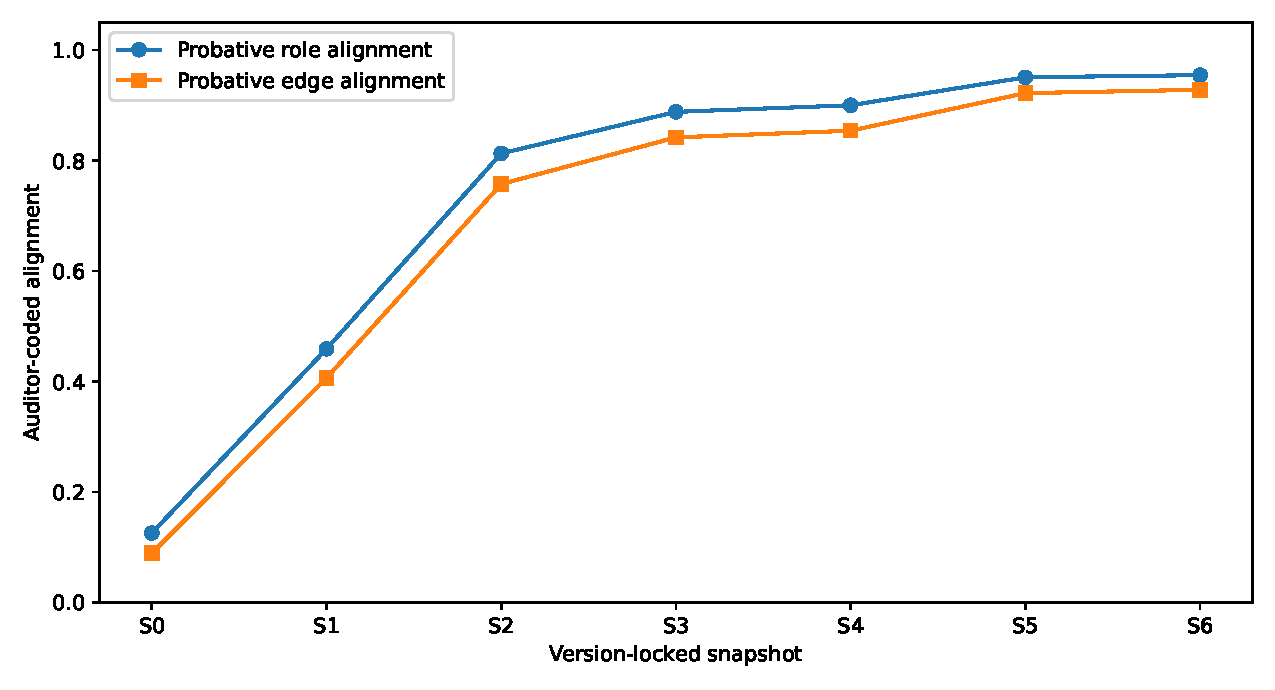
\includegraphics[width=0.91\textwidth]{../figures/structural_alignment.pdf}
\caption{Auditor-coded structural alignment across version-locked OPH
snapshots.  The curves exclude low-probative controls.  They are not
plagiarism probabilities; they quantify role and dependency-edge coverage
under the frozen public coding.}
\label{fig:alignment}
\end{figure}

Under the frozen coding, probative role alignment rises from \(0.126\) at the
1 August pre-audit public baseline to \(0.955\) at the V3.34 snapshot.  The
probative edge score rises from \(0.090\) to \(0.928\).  The largest changes
occur in the 5--7 August mechanics wave, the 12--17 August governance wave
and the 25--26 August clock/force/calibration waves, not in excluded
Born/Lorentz controls.

\subsection{The 25--26 August sequence}

Commit \texttt{4bc014ab} lands recurrence clock, charge-fixed interaction,
internal-energy inertia and local energy balance while saying that the rows
remain open and nothing is discharged.  Commit \texttt{fe4c9579} rebuilds the
flagship around a three-axiom compression thesis while naming five standing
unsupplied maps.  Commit \texttt{864051be} lands force law, speed limit,
index-versus-proper-length clock rate and a golden split, with declared
identifications, alternatives, open physical-attachment rows and explicit
falsifiers.  Its child \texttt{05207466} adds a proper-length-clocked chain,
in-block force law, golden-sector irreducibility and carrier flow, again
declaring units and clocking rules while discharging no physical row.

The inference licensed by this chronology is architectural convergence, not
subjective intent.  The appropriate next step is a dated conceptual-ancestry
statement: either exhibit a pre-contact trail for the selected ordering or
disclose material external influence, including AI context, and attribute it.

\section{Conceptual ancestry: recipe versus ingredients}
\label{sec:ancestry}

Independent code, local lemmas and implementation certificates establish
implementation authorship.  They do not by themselves establish independent
selection of the conceptual recipe: which problems are load-bearing, the
order in which they are crossed, the role each bridge plays, which
alternatives must be retained and what closes a physical claim.  We therefore
distinguish
\[
\text{independent manufacture}
\quad\text{from}\quad
\text{independent conceptual ancestry}.
\]
The public evidence ledger records directly provable dates and hashes,
role-preserving structural inferences, contextual convergences and explicit
negative controls.  It does not convert structural similarity into a legal or
intentional finding.

The requested disclosure concerns ten functions: dynamics before action;
admissible history before minimization; source/physical realization gates;
countermodels as uniqueness tests; premise ancestry and claim-status custody;
no-privilege selection; record/readout closure; observer index versus
accumulated proper history; force/current/Hamiltonian/calibration gaps; and
programme compression into a small dependency spine.  For each, a dated
pre-contact OPH trail or disclosure of external/AI-context influence would
resolve the public ancestry question far more directly than another local
proof certificate.

\section{Lean 4 proof kernel}
\label{sec:lean}

The accompanying file \texttt{PhysicalNonDefinability.lean} formalizes the
abstract logical kernel without importing OPH code.  This separation is
intentional.  The universal theorem should not depend on OPH's implementation
choices.  In addition to observational equivalence, source determination,
unique realization fibres, factorization and theorem-volume invariance, the
file now formalizes the reductio itself.  Named results include:
\begin{itemize}
\item \path{no_semantic_alchemy};
\item \path{no_source_only_enrichment_spawns_physics};
\item \path{physical_distinction_blocks_public_factorization};
\item \path{same_screen_distinct_boundary_theories_refute_screen_selector};
\item \path{same_screen_different_bulk_refutes_bare_screen_holography};
\item the concrete \path{mr_tickle_screen_reductio}.
\end{itemize}
The source also contains count-independent theorem-family blindness and
explicit 5000, 8400, 8449 and 8800 convenience corollaries.

The shortest master result is structurally:

\begin{lstlisting}
theorem no_escape_kernel
    (red : Phys -> Src) (readout : Obs -> Phys -> Val)
    {p q : Phys} {o : Obs}
    (hred : red p = red q)
    (hsep : readout o p != readout o q) :
    not (SourceDetermines red (ObsEq readout))
\end{lstlisting}

An ASCII rendering appears in \cref{app:lean}; the exact UTF-8 Lean source accompanies the article.  The present build
environment did not contain a Lean executable, so the article does not
represent the supplement as compiled here.  Its statements use only elementary
Lean 4 definitions and are deliberately small enough for independent checking.

\section{Discussion}

\subsection{Why one metatheorem outweighs a large proof surface}

A proof assistant checks whether conclusions follow from encoded premises.  It
does not decide whether the premises are physically necessary, whether a
formal object has the claimed laboratory meaning, or whether an unencoded
realization map is unique.  Thus a large theorem count can coexist with a
single missing physical bridge.

The appropriate comparison is not
\[
\text{number of lemmas versus number of lemmas},
\]
but
\[
\text{source theory}\quad\longrightarrow\quad
\text{realization fibre}\quad\longrightarrow\quad
\text{physical readouts}.
\]
If the middle fibre is non-singleton, every source-internal proof leaves the
physical ambiguity untouched.

\subsection{Why the theorem is not anti-formalization}

Formalization is especially valuable here.  It prevents a theory from moving
silently between source structure and physical interpretation.  The no-go
suite should be imported alongside OPH's own modules and instantiated with
its exact source-reduct function, physical-realization type and readout family.
A successful OPH reply would be a formal uniqueness theorem.  A failed
instantiation would identify the exact additional premise required.

\subsection{Relation to underdetermination in physics}

Physical theories routinely share local algebraic data while differing in
global structure, couplings, matter content, topological sectors or line
operators.  The global-form example in gauge theory is not a philosophical
possibility but standard field-theoretic structure~\cite{AharonySeibergTachikawa}.
The no-go theorem therefore does not impose an artificial standard.  It asks a
reconstruction programme to distinguish alternatives that established physics
already distinguishes.

\subsection{Strongest defensible status for OPH after the reductio}

At the frozen commit, OPH's own seven-value status discipline can absorb the
result cleanly:

\begin{itemize}
\item source-internal universal results may be \texttt{axiom\_forced};
\item exhaustively checked finite constructions may be
\texttt{exact\_named\_realization};
\item unclosed lifts remain \texttt{conditional\_open\_interface};
\item countermodel-limited statements are \texttt{independence\_limited};
\item laboratory mappings are \texttt{physical\_identification}.
\end{itemize}

The no-go demands that these distinctions govern headline claims as well as
registries.  If they do, OPH is a conditional reconstruction programme with a
large formal apparatus.  If they do not, the broader physical claim is not
entailed by the frozen axioms.

\section{Conclusion}

The Mr Tickle Screen makes the foundational issue difficult to disguise.  A
formal source structure can be represented on a scientific-looking sphere, on
a long-armed orange cartoon, or in a text file.  If those presentations carry
the same protected source structure, source theorems cannot distinguish them.
Nothing about one presentation causes nature to instantiate its referent.
That missing relation is external to source syntax unless physical semantics
has been imported as additional structure.

The result is exact.  \emph{No Semantic Alchemy} proves that no satisfiable
source-only enrichment can force an unconstrained external realization
relation to be inhabited.  \emph{No boundary theory from bare screen} proves
that one finite carrier can support inequivalent boundary dynamics.  \emph{No
Bulk From Bare Boundary} proves that a bulk assignment cannot factor through a
bare screen when those boundary theories reconstruct differently.  HKLL and
related holographic machinery do not rescue the bare screen: they begin with a
specified boundary quantum theory and a reconstruction dictionary, precisely
the objects that bare incidence and observer consensus do not supply.

For OPH, the strongest rigorous conclusion is therefore stronger than ``some
physical bridges remain open.''  As long as the programme remains a
source-only derivation from A1--A3 and their formal consequences, physical
closure is impossible.  A future successful physical closure would have to
supply independently grounded boundary dynamics, physical realization,
calibration and a valid holographic dictionary.  Those additions could make a
new theory scientifically substantive, but they would also identify the
load-bearing physical structure that the original three-axiom screen did not
contain.

Thus the final no-escape statement is
\[
\boxed{
\text{formal screen}
\not\Rightarrow
\text{physical boundary theory}
\not\Rightarrow
\text{holographic dictionary}
\not\Rightarrow
\text{physical bulk}.}
\]
The crossed arrows are not invitations to add more decorative source
formalism.  Each is a separate existence/uniqueness/realization obligation.
Looking harder at the drawing does not put a universe behind it.

\section*{Methods}

\paragraph{Repository audit.}
The OPH basis was frozen to the commit stated in \cref{sec:versionlock}.  The
reader-facing axiom reference and README were treated as primary public
sources.  No inference in the theorem suite depends on mutable branch-head
language after that hash.

\paragraph{Formal method.}
The proof separates a source signature from a physical extension signature,
forms the reduct functor, and defines physical uniqueness as observational
singleton fibres.  Standard reduct invariance supplies the core
indiscernibility result.  Beth definability is used only as an additional
first-order closure; the direct two-expansion proof applies more generally.

\paragraph{Physical witness discipline.}
A counterexample counts only when the models share the frozen source reduct
and differ in an admitted gauge-invariant readout.  Differences of notation,
coordinates, labels or hidden implementation do not qualify.

\paragraph{Holographic typing audit.}
The holography section uses Maldacena/Witten/HKLL/ADH only for the established
typing of the reconstruction problem: a specified boundary quantum theory and
duality/reconstruction data precede the reconstruction of bulk operators.  No
claim is made that HKLL itself proves ontological reality.  The audited claim
is narrower: a bare finite screen is not, by itself, the boundary quantum
theory that HKLL consumes.

\paragraph{Live-head separation.}
The theorem is proved against a frozen baseline so later changes cannot be
projected backward.  A separate 26 August public-head snapshot is cited only
to show that the current programme still advertises an emergent-reality/
holographic-screen reconstruction and a theorem count exceeding 8800.

\section*{Data and code availability}

The primary manuscript source and abstract Lean 4 theorem kernel accompany
this article.  The audited OPH source is publicly versioned by the frozen Git
commit.  The author's 2 August 2026 featureless countermodel is preserved as
both LaTeX and PDF with hashes recorded in the associated provenance dossier.

\section*{Author contributions}
The public package is issued anonymously.  The technical audit, role coding,
source custody and formal kernel are open to public correction through the
repository workflow.

\section*{Competing interests}

The author declares no financial competing interests.  This article is an
adversarial scientific audit of a public theoretical programme and is not a
legal adjudication of authorship or intent.

\clearpage
\appendix

\section{Formal response checklist}
\label{app:checklist}

For each disputed OPH claim \(C\), a reproducible audit should publish:

\begin{enumerate}
\item frozen commit and file hashes;
\item complete dependency list for \(C\);
\item source signature \(\Lsrc\);
\item physical extension signature \(\Lphys\);
\item reduct map \(U\);
\item physical realization relation or functor;
\item admitted physical readout family \(\Obs\);
\item proof of existence of a physical lift;
\item proof of observational uniqueness of the lift;
\item countermodel search over alternative lifts;
\item explicit classification of every added premise;
\item statement of the strongest surviving claim if uniqueness fails.
\end{enumerate}

A response that omits items 3--9 has not answered the theorem.  It has changed
vocabulary without closing the realization fibre.

\section{Lean 4 theorem kernel}
\label{app:lean}

\VerbatimInput[fontsize=\scriptsize,breaklines=true,breakanywhere=true,frame=single,framesep=2mm]{PhysicalNonDefinability_ascii_v3.txt}

\clearpage
\begin{thebibliography}{99}

\bibitem{AnonFeatureless}
Anonymous prior audit, \emph{Algebraic Recovery Without Physical Realization: A
Featureless Model of the Gauge-Source Interfaces in Observer Patch
Holography} (2 August 2026).  Preserved manuscript SHA-256:
\texttt{44e61768568416c08255b951497c3ba0c8fc131501b240967175ab21100c1e7d}.

\bibitem{OPHAxiomReference}
B. M\"uller and contributors, \emph{The OPH Axiom Reference},
FloatingPragma/observer-patch-holography, commit
\texttt{40b13bb4bc56261f84fd515701916c388c42fe83} (26 August 2026),
\url{https://github.com/FloatingPragma/observer-patch-holography/blob/40b13bb4bc56261f84fd515701916c388c42fe83/docs/AXIOM_REFERENCE.md}.

\bibitem{OPHCurrentREADME}
B. M\"uller and contributors, \emph{Observer Patch Holography}, README at
main-branch snapshot \texttt{05207466cf63461c683bf1b8543d7c4a5feea4fa}
(26 August 2026),
\url{https://github.com/FloatingPragma/observer-patch-holography/blob/05207466cf63461c683bf1b8543d7c4a5feea4fa/README.md}.

\bibitem{OPHArchivedHolography}
B. M\"uller and contributors, \emph{Why Holography Looks Like a Boundary},
archived OPH book chapter at snapshot
\texttt{05207466cf63461c683bf1b8543d7c4a5feea4fa},
\url{https://github.com/FloatingPragma/observer-patch-holography/blob/05207466cf63461c683bf1b8543d7c4a5feea4fa/archive/book-v1/chapter-08-holography.md}.

\bibitem{Maldacena1997}
J. M. Maldacena, The large \(N\) limit of superconformal field theories and
supergravity, \emph{Advances in Theoretical and Mathematical Physics}
\textbf{2}, 231--252 (1998), arXiv:hep-th/9711200.

\bibitem{Witten1998}
E. Witten, Anti-de Sitter space and holography,
\emph{Advances in Theoretical and Mathematical Physics} \textbf{2}, 253--291
(1998), arXiv:hep-th/9802150.

\bibitem{HKLL2006}
A. Hamilton, D. Kabat, G. Lifschytz and D. A. Lowe,
Local bulk operators in AdS/CFT: a boundary view of horizons and locality,
\emph{Physical Review D} \textbf{73}, 086003 (2006),
doi:10.1103/PhysRevD.73.086003, arXiv:hep-th/0506118.

\bibitem{ADH2015}
A. Almheiri, X. Dong and D. Harlow, Bulk locality and quantum error correction
in AdS/CFT, \emph{Journal of High Energy Physics} \textbf{2015}, 163 (2015),
doi:10.1007/JHEP04(2015)163, arXiv:1411.7041.

\bibitem{Beth1953}
E. W. Beth, On Padoa's method in the theory of definition,
\emph{Indagationes Mathematicae} \textbf{15}, 330--339 (1953).

\bibitem{Hodges1993}
W. Hodges, \emph{Model Theory} (Cambridge University Press, Cambridge, 1993).

\bibitem{ChangKeisler}
C. C. Chang and H. J. Keisler, \emph{Model Theory}, 3rd edn
(North-Holland, Amsterdam, 1990).

\bibitem{KullbackLeibler}
S. Kullback and R. A. Leibler, On information and sufficiency,
\emph{Annals of Mathematical Statistics} \textbf{22}, 79--86 (1951).

\bibitem{Csiszar1975}
I. Csisz\'ar, \(I\)-divergence geometry of probability distributions and
minimization problems, \emph{Annals of Probability} \textbf{3}, 146--158
(1975), doi:10.1214/aop/1176996454.

\bibitem{Jaynes1957}
E. T. Jaynes, Information theory and statistical mechanics,
\emph{Physical Review} \textbf{106}, 620--630 (1957).

\bibitem{AharonySeibergTachikawa}
O. Aharony, N. Seiberg and Y. Tachikawa, Reading between the lines of
four-dimensional gauge theories, \emph{Journal of High Energy Physics}
\textbf{2013}, 115 (2013), doi:10.1007/JHEP08(2013)115.


\bibitem{Shannon1948}
C. E. Shannon, A mathematical theory of communication,
\emph{Bell System Technical Journal} \textbf{27}, 379--423 and 623--656
(1948).

\bibitem{OPHTheoremFloor}
B. M\"uller and contributors, commit
\texttt{4bc014ab838bf98b1d8c0b517c087d7df10ce73e},
\emph{Land the core-physics wave: recurrence clock, charge-fixed interaction,
internal-energy inertia, local energy balance},
FloatingPragma/observer-patch-holography (25 August 2026).  The commit message
states ``raise the theorem floors to 8400.''

\bibitem{Lean4}
L. de Moura and S. Ullrich, The Lean 4 theorem prover and programming
language, in \emph{Automated Deduction -- CADE 28}, Lecture Notes in Computer
Science \textbf{12699}, 625--635 (Springer, 2021),
doi:10.1007/978-3-030-79876-5\_37.

\bibitem{PeskinSchroeder}
M. E. Peskin and D. V. Schroeder, \emph{An Introduction to Quantum Field
Theory} (Addison-Wesley, Reading, MA, 1995).

\end{thebibliography}

\end{document}
